\documentclass[11pt]{article}
\usepackage[utf8]{inputenc}
\usepackage{amsmath,setspace,geometry}
\usepackage{amsfonts}
\usepackage[shortlabels]{enumitem}
%\usepackage[dvipdfmx]{hyperref,graphicx}
\usepackage{graphicx}
\usepackage{bbm}

\usepackage[colorlinks,citecolor=purple,urlcolor=blue,bookmarks=false,hypertexnames=true]{hyperref}
\usepackage[]{natbib} 
\bibpunct[:]{(}{)}{,}{a}{}{,}
\geometry{left = 1.0in,right = 1.0in,top = 1.0in,bottom = 1.0in}
%\onehalfspacing
% \usepackage{setspace}
\doublespacing
%\renewcommand{\baselinestretch}{0.3}
\usepackage[english]{babel}
\usepackage{float}
\usepackage{booktabs}
\usepackage{pdfpages}
\usepackage{threeparttable}
\usepackage{lscape}
\usepackage{subfig}
%\setstretch{1.2}
\newtheorem{assumption}{Assumption}
\newtheorem{definition}{Definition}
\newtheorem{example}{Example}
\newtheorem{lemma}{Lemma}

\title{Unified Container Shipping Industry Data From 1966: Freight Rate, Shipping Quantity, Newbuilding, Secondhand, and Scrap Price\thanks{ Declarations of interest: none}}
\author{Takuma Matsuda\thanks{Faculty of Commerce, Takushoku University. Email: tmatsuda@ner.takushoku-u.ac.jp}\quad  Suguru Otani\thanks{Department of Economics, Rice University. Email: so19@rice.edu}}
\date{
First version: November 29, 2022\\
Current version: \today
}

\begin{document}

\maketitle

\begin{abstract}
We constructed a new unified panel dataset of route-year-level freight rates and shipping quantities for the six major routes and industry-year-level newbuilding, secondhand, and scrap prices from 1966 (beginning of the industry) to 2009. We provide detailed guidance on how to merge multiple datasets and verify the consistency of the data with the historical knowledge and experience of industry experts and former executives. Using this data, we provide a descriptive analysis of quantitatively unknown industry dynamics known as the container crisis. Finally, we detect structural breaks for each variable to illustrate the effect of the breakdown of shipping cartels.
\end{abstract} 

\vspace{0.1in}
\noindent\textbf{Keywords:} container shipping industry; exemption agreement; container crisis; shipping cartel; container freight rate 
\vspace{0in}
%\newline
%\noindent\textbf{JEL Codes:} C78, L11, L25, L41, L50, L91

%\tableofcontents

{\flushright{``When we think about technology that changes the world, we think about glamorous things like the Internet. But if you try to figure out what happened to world trade, there is a strong case to be made that it was containers.”\\
-- Krugman, Paul.\footnote{Citigroup Foundation Special Lecture, Festschrift paper in honor of Alan V. Deardorff, University of Michigan IPC working paper 91, 2009}\\
``[W]ithout [the container], the tremendous expansion of world trade in the last forty years—the fastest growth in any major economic activity ever recorded—could not possibly have taken place.”\\
-- Drucker, Peter F.\footnote{Innovation and Entrepreneurship, Butterworth-Heinemann, 2007 (p.28)}}
\flushright{}}

\section{Introduction}\label{sec:introduction}

Container shipping is the bloodstream of global trade and technology that have changed the world. According to IHS Markit and Descartes Datamyne, 45.4\% of the amount-based import to the U.S., 21.3\% of the amount-based export from the U.S., and 10.12\% of quantity-based world trade are shipped by container shipping in 2021. Also, the container shipping industry is a fascinating laboratory for investigating industry dynamics. Because the industry started a global shipping business in 1966, we can determine the initial state of the market dynamic structure with substantial firm entry and exit. Another feature is that many countries have exemption agreements that include international cartels and consortia in their competition laws.\footnote{\cite{Anteitekina_kokusaikaijouyusoukakuhonotameno_kaijiseisakuno_arikatanitsuite2007} of the Ministry of Land, Infrastructure and Transportation in Japan defines a shipping conference as an agreement on freight rates and other business matters to restrain competition among container shipping lines along the same route. A consortium is a technical agreement between several shipping lines to form a group and operate a joint service for the diversification of services and cost reduction in the liner service. Consortiums include alliances that are widely used. } In the shipping industry, international shipping cartels are called  ``shipping conferences."\footnote{There is an important difference between shipping conferences and alliances: conferences are organized by specific routes and directions, while alliances are formed globally. There may exist one conference covering trade on the Transatlantic route and another covering trade between Northern Europe and the U.S. Gulf ports. In addition, firms do not always participate in conferences on all routes and directions they serve. Thus, conferences are heterogeneous in their structure and membership.} Despite the significance, there is a lack of a panel dataset for the route-year-level freight rate and shipping quantity in the container shipping industry, notably for the years 1966 to 1990; therefore, quantitative research for this period is limited.\footnote{As other related studies focus on the container freight rate panel data, \cite{luo2009econometric} use shipping demand and freight rate data between 1980 and 2007. As shipping demand, they used the world container throughput reported in the Drewry Annual Container Market Review and Forecast. The container freight rate is calculated as the weighted average of the Transpacific, Europe-Far East, and Transatlantic trades from the same data source. Due to data limitations, they calculated the missing period (1980–1993) from the General Freight Index in the Shipping Statistics Yearbook 2007, using a simple statistical equation between the container freight rate and the general freight index from 1994 to 2008.} This study offers the unified dataset based on published books and publicly available data sources to the extent possible. Additionally, we combine route-year-level data with new industry-level data regarding shipbuilding, secondhand, and scrap prices.\footnote{The data sources are listed in Appendix \ref{sec:data_construction}.} 

We have adopted the tractable imputation approach, that is, linking multiple data sources, which overlaps information for some years, instead of constructing the freight index manually from the commodity-level freight rate via formal but complicated processes or taking an estimation approach assuming the AR(1) process under stationary assumption \citep{jeon2022learning}. We have also checked the validity by presenting interview-based evidence from ex-executive officers of shipping companies. This confirms that our Twenty-foot Equivalent Unit (TEU)-based price data provides a reasonable benchmark measure, although container freight rates were not determined by container units in the 1970s.

Using our new dataset, we implemented the unknown multiple structural breaks test \citep{bai1998estimating,bai2003computation} to analyze historical shipping price reductions in the 1980s known as the ``container crisis" \citep{broeze2002globalisation}. It has been anecdotally known that the crisis was triggered by the two events: (1) the withdrawal of Sea-Land, which was the biggest cartel member from shipping cartels in 1980, and (2) the enactment of the Shipping Act of 1984. The first event changed the market share of shipping cartels, whereas the second event neutralized the shipping cartels. We also applied the test to industry-year-level newbuilding, secondhand, and scrap prices to determine the relationship between shipping markets and shipbuilding markets.

Given the test, first, we found that the container crisis occurred on all six routes by 1980, which was triggered by the withdrawal of Sea-Land, although non-U.S. routes reacted earlier than U.S. routes. Second, we found that industry-year-level newbuilding, secondhand, and scrap prices displayed a relatively stable trend during the container crisis, unlike shipping prices. We interpret these differences as naturally capturing the differences between shipping markets with shipping conferences and shipbuilding markets without cartel groups. Thus, the container crisis was a specific event in the shipping market.


\subsection{Literature review}\label{subsec:litereture}

This study contributes to two strands of the literature: the historical connection to the recent growing empirical research on the shipping industry and the effect of an explicit cartel on the price in the shipping industry.

First, this study provides the necessary data to connect the history of the container shipping industry from its beginning to its development after 2000, which has gained attention in the industrial organization literature  \citep{aguirregabiria2021dynamic}. The most relevant paper was \cite{jeon2022learning}. She examined the relationship between demand uncertainty and firm-market-year-level investment decisions using container shipping demand and freight rate data for the years 1997 to 2014. To facilitate her learning-based model, she needed to obtain the initial prices and demand in the container industry. Because of her data limitations, she took imputation and truncation approaches for missing shipping demand data from 1966: Q2 to 1996: Q4.\footnote{On cartel issues in a similar industry, the most relevant paper is by \cite{asker2010leniency}. He studied how the presence of a cartel affects market conduct following its dissolution and how the dissolution might be affected by the obligations imposed on firms that seek leniency in the tanker shipping market between 2001 and 2002. \cite{kalouptsidi2014aer}, \cite{brancaccio2020geography}, and \cite{greenwood2015waves} investigated the bulk shipping industry after 2000. \cite{bai2021congestion} studied the tanker market during 2017-2020 and investigated how the imbalance between the demand for and the supply of shipping services
determines congestion. Although these industries are closely related to the container shipping industry, each of the industries is characterized differently because the market structure and competition are different. In addition, \cite{kalouptsidi2017res} and \cite{barwick2019china} studied the shipbuilding industry, which is an upstream industry for the container and bulk shipping industries. These papers rely on the use of Clarksons Research database and focus on the period after 2000. In the literature on international trade, \cite{bernhofen2016estimating} use country-level panel data regarding containerization adoption for the period 1962–1990. They focused on the effect of containerization adoption on the trade quantity; therefore, they refer to \textit{the Containerization International Yearbook} only for obtaining the first presence of container technology in each country. \cite{rua2014diffusion} added port-level data to their study and investigated the diffusion of initial adoptions of containerized transportation. \cite{cocsar2018shipping} exploited rich Turkish export data and examined modal choice between containerization and breakbulk shipping.} Our study overcomes this limitation and complements the findings of previous studies.



Second, this study detects the effect of explicit shipping cartels on shipping prices.\footnote{%See a companion paper \citep{matsuda2022disentangling} for reference of structural estimation results with institutional details.
The ongoing study of one of the authors of this paper investigates the effect by constructing a structural model and focuses on the shipping conferences as a single explicit cartel entity, and departs from the traditional focus on tacit collusion in the literature, e.g., \cite{porter1983study}, \cite{bresnahan1987competition}, \cite{miller2017understanding}, and \cite{byrne2019learning}.
%\textcolor{blue}{Otani (2022) also incorporates dynamic investment decisions with the cartel mechanism and unobserved correlated productivity.}
The institutional background is similar to \cite{igami2015market}'s findings. He studied the impact of market power on international coffee prices and evaluated the impact of a cartel treaty on coffee prices and its global welfare consequences under counterfactual competition regimes, that is., collusion versus Cournot–Nash in a single homogenous good market.} Shipping cartels have been recognized in survey papers, such as those by  \cite{levenstein2006determines}, and \cite{asker2021}. Some studies, such as those of \cite{morton1997entry} and \cite{podolny1999social}, examine specific shipping cartels in the U.K. in the 1800s. The most relevant studies are those by  \cite{wilson1991some}, \cite{pirrong1992application}, and \cite{clyde1998market}. \cite{wilson1991some} provided evidence of regime change by the Shipping Act of 1984 using data on quarterly freight rates and shipping quantities of the five selected commodities only on the Transpacific route.  \cite{pirrong1992application} tested the model prediction of the core theory surveyed in \cite{sjostrom2013competition} using the data of two specific trade routes between 1983 and 1985. \cite{clyde1998market} studied the relationship between market power and the market share of shipping conferences after the act. However, they did not exploit cross-sectional variations, especially between non-U.S. and U.S. routes. Our data contain cross-sectional variations in the freight rates. Thus, to the best of our knowledge, owing to data limitations, our study is the first empirical research to detect the effect of shipping cartels on the six main routes after global containerization in the 1970s.

The remainder of this paper is organized as follows. Section \ref{sec:data} summarizes the data and institutional background of the container shipping industry. Section \ref{sec:interview} presents the interview-based evidence of an ex-chairperson and an ex-vice chairperson to demonstrate the consistency of our recovered data. Section \ref{sec:structural_break_test} implements structural break tests to detect price reductions in market variables. Section \ref{sec:conclusion} presents our conclusions. Appendix \ref{sec:data_construction} presents the details of data construction.

\section{Data and Institutional Details}\label{sec:data}

We provide details of the data source in Section \ref{subsec:data}. Next, we provide graphical interpretations in Section \ref{subsec:graphical_interpretation} and summary statistics of the variables in Section \ref{subsec:summary_statistics}. Then, we introduce the institutional details. For clarification, a \textit{market} in this industry is a nondirectional location pair, that is, if a firm operates a container ship in the eastbound of the transpacific, then it should operate the ship in the westbound. A \textit{route} is a directional round-trip between two locations, for example, both westbound and eastbound of the transpacific. An \textit{industry} is an entire market consisting of all six routes.

\subsection{Data source}\label{subsec:data}
We constructed route-year-level and industry-year-level data of the container shipping industry.\footnote{Based on the firm-level data, each route is divided into conference and non-conference routes. For example, the Transatlantic eastbound conference route is a single route and the Transatlantic conference market is a single market. A conference market is a market where all conference firms conducted collusive behavior under the shipping conferences before the Shipping Act, but have competed since the act, whereas a non-conference market is a market where all non-conference firms have competed throughout the whole period. In the interview with ex-practitioners in shipping companies, they told that container freight rates for nonmember carriers are 20\% to 30\% lower than conference firms on the same routes. However, as far as we know, there was no data available on the trends in freight rates offered by the non-conference carriers. In addition, although we checked \textit{The Japan Maritime Daily}, the newspaper of the maritime industry, we could not find any articles that continuously reported on the level of freight rates offered by the non-conference carriers. } First, we used route-year-level data of the container freight rate and shipping quantity. Collecting data, particularly before 1994, was not trivial because there is no single data source that covers the period between 1966 and 1993. Thus, we needed to carefully combine data from multiple sources carefully.\footnote{For reference, we merge \textit{``Issues of Our Ocean Shipping"} (\textit{``Wagakuni no Gaikou Kaiun Ni Tsuite," in Japanese}), \textit{Global Container Markets Drewry Shipping Consultants}, \textit{Review of Maritime Transport}, \textit{Containerization International 1973}, \textit{World Sea Trade Service}, \textit{Container transportation cost and profitability 1980/2000}, \textit{The Container Crisis 1982}, \textit{World Container Data 1985}, and \textit{World's sea trades}. Then, we converted merged data into TEU-based data.} In Appendix \ref{sec:data_construction}, we provide the data source and a detailed guide with some assumptions on data construction for each container freight rate and shipping quantity on six major routes: mainhaul and backhaul (separately) on the Transpacific (Asia and North America), Transatlantic (North America and Europe), and Asia-Europe routes. Finally, we use price and quantity data in the six routes between 1966 and 2009. The price was adjusted according to the CPI in the U.S. in 1995. To check the accuracy and validity, in Section \ref{sec:interview}, we provide interview-based evidence on the consistency of our recovered data with the historical experience of industry experts, Akimitsu Ashida and Hiroyuki Sato.

Second, we used industry-year-level data for newbuilding, secondhand, and scrap prices.\footnote{For reference, we merge \textit{Review (1971-1998)} and \textit{Lloyd's Shipping Economist (1983-1990)}. Then, we convert merged data into TEU-based data.} Finally, we used the newbuilding and scrap prices per TEU between 1966 and 1998 and the secondhand price per TEU between 1968 and 1998. Prices were adjusted to the CPI in the U.S. in 1995. 

Note that recent data on newbuilding, secondhand, and scrap prices after 1998 and shipping prices and quantities after 2009 are sold by companies such as Clarksons and IHS Markit. Our data can be merged with proprietary data. This study does not include proprietary data to share our data for public use.

\subsection{Graphical interpretation}\label{subsec:graphical_interpretation}
\subsubsection{Route-year-level shipping price and quantity data}



Figure \ref{fg:container_freight_rate_and_shipping_quantity_each_route} illustrates the nonstationary trends in the container freight rate and shipping quantity between 1966 and 1990. The container freight rate decreased with fluctuations, and suddenly dropped significantly. As a remarkable feature, the transition of freight rates on Asia-Europe eastbound (Europe to Asia) and westbound (Asia to Europe) routes is more unstable than those on Transpacific and Transatlantic routes in the 1970s and the 1980s. This might be because the strength of the shipping conference on the Asia-Europe route decreased, and its impact was more significant.\footnote{In the interview with an ex-executive of a Japanese shipping company, he pointed out the difference between conferences. Conferences related to Asia-Europe had a strict membership screening process, and the number of voyages by member companies was clearly defined (closed conference). In addition, some members in the conference pooled their freight and then redistributed them. In contrast, the conferences for Transpacific routes were free to join or leave (open conference), and freight pooling was explicitly prohibited under the Shipping Act of 1916 in the U.S.} 

The shipping quantity on all routes increased monotonically between 1973 and 1990. In particular, after 2000, shipping quantity trend increased exponentially in the Transpacific eastbound and Asia-Europe eastbound routes due to the surge in imports from Asian countries, especially China. \cite{jeon2022learning} investigated these features in detail these features after 2000. 

The enactment of the Shipping Act of 1984 in the US divided the conference market regime sharply before and after 1984, as illustrated by the trend of the container freight rate in Figure \ref{fg:container_freight_rate_and_shipping_quantity_each_route}. Under the legislation of the Shipping Act of 1984 in the U.S., shipping conferences were much easier to form. Also, after 1984, the Transpacific and Transatlantic routes experienced severe price reductions via market competition.\footnote{This is consistent with an interview article to ex-executives of Japanese shipping companies \citep{JapanMaritimeDaily2006} that were in charge of container trades in the 1980s.} The change in the market regime shaped the container crisis.



\begin{figure}[!ht]
\begin{center}
  \subfloat[Price]{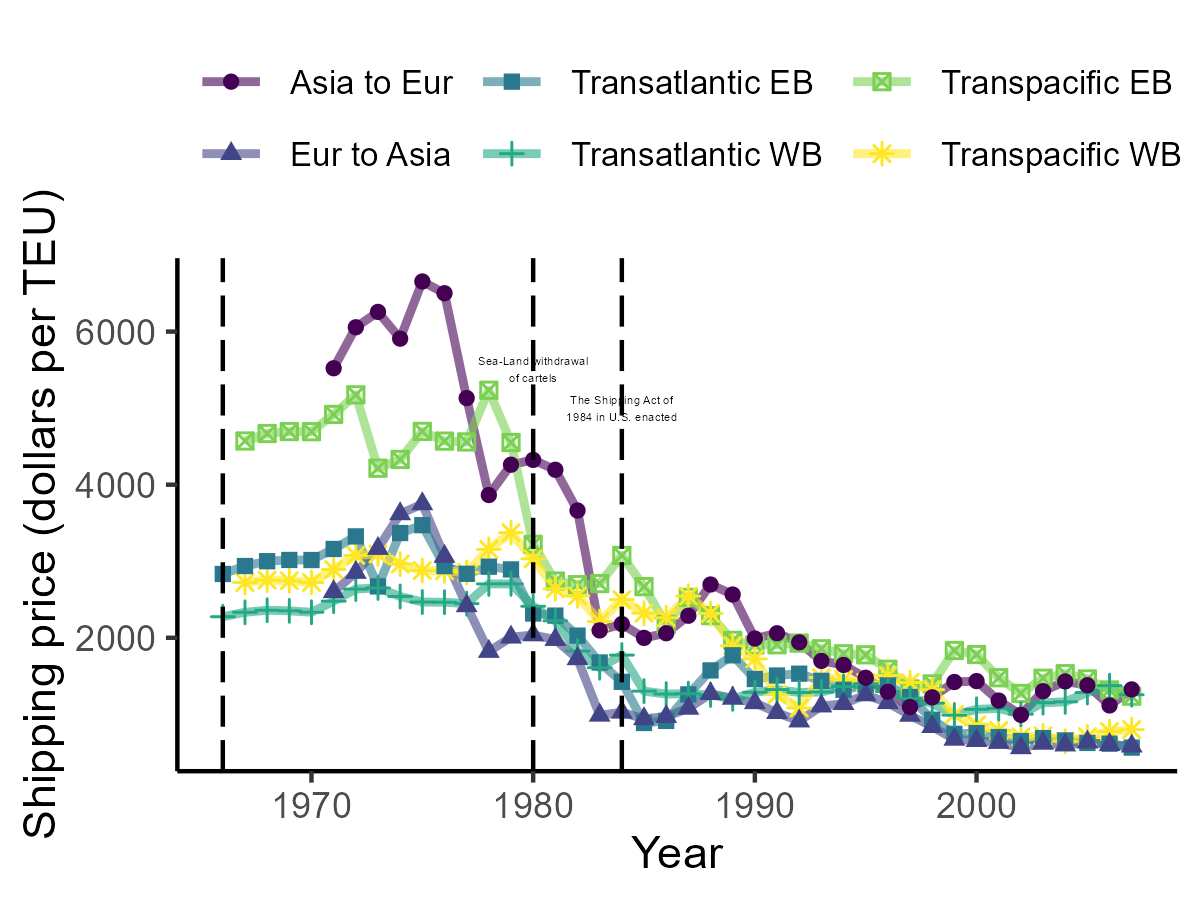
\includegraphics[width = 0.7\textwidth]
  {figuretable/container_freight_rate_each_route.png}}\\
  \subfloat[Quantity]{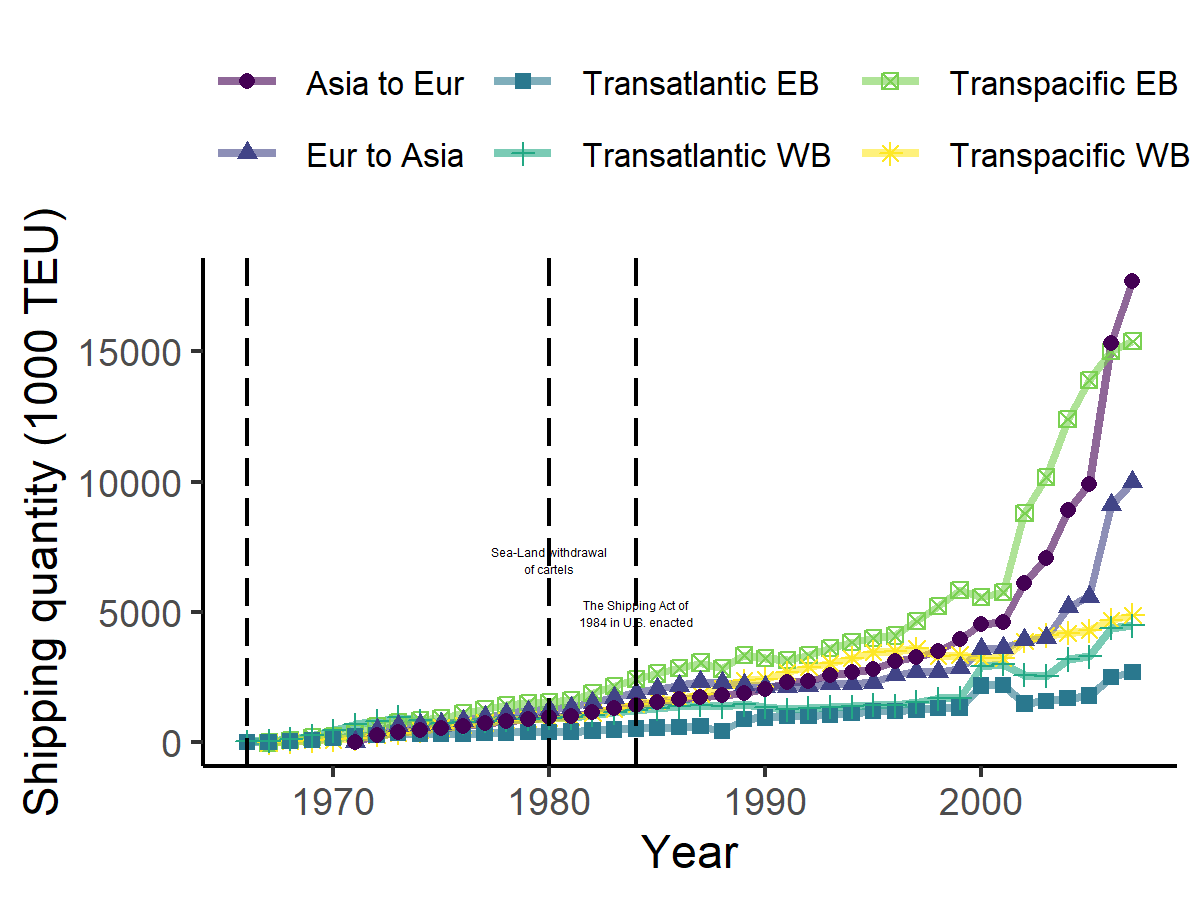
\includegraphics[width = 0.7\textwidth]
  {figuretable/container_shipping_quantity_each_route.png}}
  \caption{Trends in route-year-level shipping prices and quantities.}
  \label{fg:container_freight_rate_and_shipping_quantity_each_route}
  \end{center}
\footnotesize
  Note: Container freight rates before 1992 refer to conference prices. The container freight rates after 1993 are unified prices based on conference and non-conference  prices, and the difference between them is known to vanish because of the Shipping Act of 1984. The latter are standard data often used in the literature, such as \cite{jeon2022learning}. Prices were adjusted to the CPI in the U.S. in 1995.
\end{figure}


\subsubsection{Industry-year-level newbuilding, secondhand, and scrap prices data}


\begin{figure}[!ht]
\begin{center}
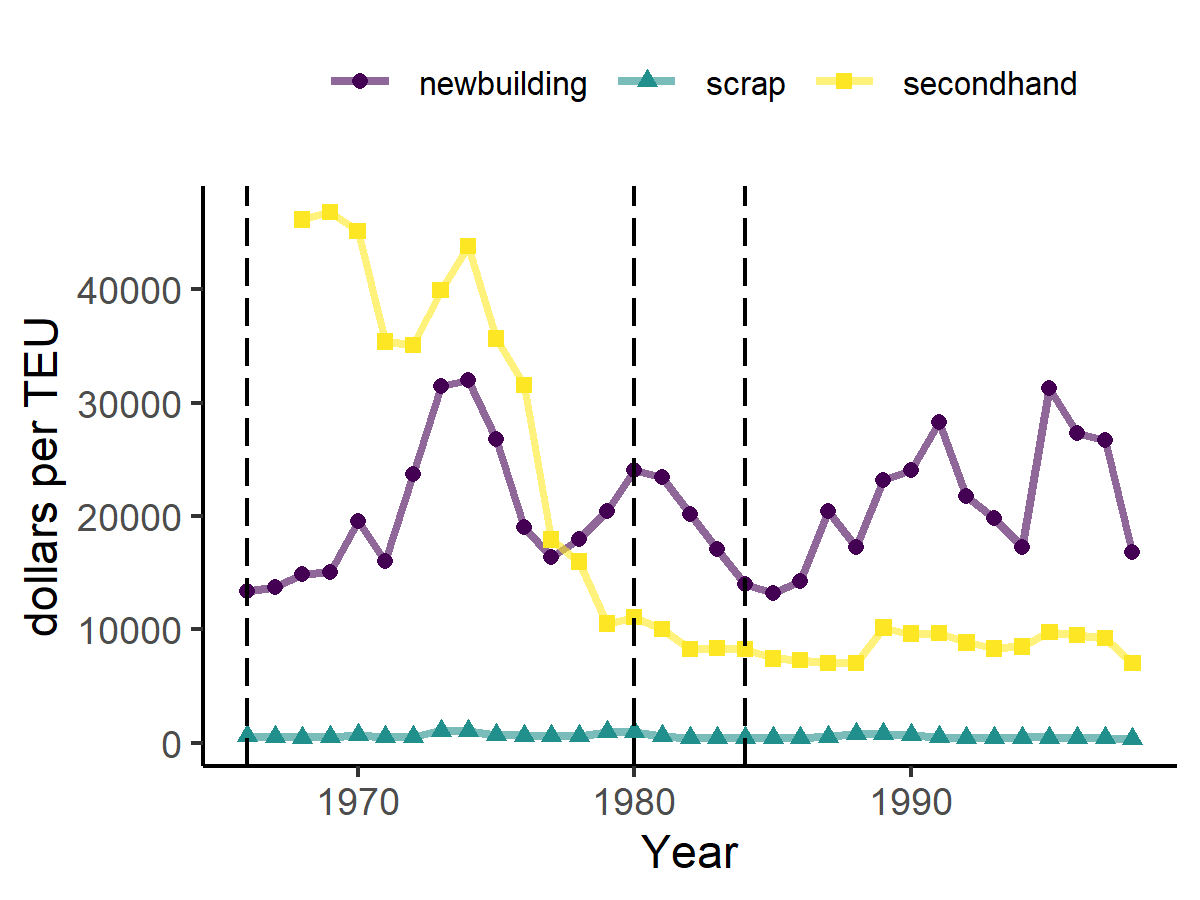
\includegraphics[width = 0.7\textwidth]{figuretable/price_newbuilding_secondhand_scrap.png}
\caption{Trends in industry-year-level newbuilding, secondhand, and scrap prices.}
\label{fg:price_newbuilding_secondhand_scrap}
\end{center}
\footnotesize
The data span 33 years (1966-1998) for the entire container shipping industry. The data cover newbuilding and scrap prices between 1966 and 1998 and secondhand prices between 1968 and 1998. All prices were adjusted according to the CPI in the U.S. in 1995. 
\end{figure}

Figure \ref{fg:price_newbuilding_secondhand_scrap} illustrates the transitions of newbuilding, secondhand, and scrap prices. First, we observe four peaks in the newbuilding price in 1974, 1980, 1987, and 1991, which indicates that the newbuilding price shows peaks at similar timings to the shipping price. Surprisingly, the shipping price after adjusting CPI did not decrease significantly, which means that the trend of newbuilding price was not downward unlike shipping price. This is a new finding because it is anecdotally known that the ship itself was expensive in the 1970s and the shipbuilding price per TEU decreased in the 1990s due to the gradual increase in the size of ships.\footnote{When Sea-land began container transport services in 1966, 226 35-foot containers were deployed. In the 1970s, with the development of international maritime container transport, container vessels began to increase in size, with vessels of approximately 2,000 TEU becoming the mainstay of liner services. Owing to increased competition following the Shipping Act of 1984, shipping companies wanted to introduce even larger vessels. In 1988, American President Lines (APL) opened a 39.1-meter wide, 4,300 TEU vessel, the first container vessel that could not pass the Panama Canal. Further, in the 1990s, 6,000TEU-class vessels come into the container shipping market.} We find that increasing CPI corresponds with seemingly decreasing shipbuilding price in the nominal sense. 

Second, the secondhand price decreased sharply between 1974 and 1979. On the other hand, the price after 1980 was stable relative to shipping and newbuilding prices. In the 1970s, full container vessels began to operate on liner routes, and the number of vessels was insignificant. Therefore, the number of vessels traded in the secondhand market was small, and there was supposed to be more fluctuation in secondhand prices. On the other hand, since the 1980s, the number of vessels being traded in the secondhand market has increased, leading to stable secondhand freight rates and a more vital linkage with new building prices.

Third, the scrap price is stable, without any large fluctuation relative to the other price variables. Also, the level of the scrap price is smaller than the newbuilding and secondhand prices because the scrap price corresponds with the input price such as a steel price in itself. Thus, the trend reflects the dynamics of the input price.


% \begin{figure}[!ht]
%   \begin{center}
%   \subfloat[Transpacific]{\includegraphics[width = 0.32\textwidth]
%   {figuretable/cartel_level_share_transition_transpacific.png}}
%   \subfloat[Transatlantic]{\includegraphics[width = 0.32\textwidth]
%   {figuretable/cartel_level_share_transition_transatlantic.png}}
%   \subfloat[Asia-Europe]{\includegraphics[width = 0.32\textwidth]
%   {figuretable/cartel_level_share_transition_asia_and_europe.png}}
%   \caption{Conference and non-conference market shares}
%   \label{fg:cartel_level_share_transition_asia_and_europe}
%   \end{center}
%   \footnotesize
%   Note: Conference and non-conference market shares are calculated by the tonnage share of ships deployed in the westbound and eastbound of the market. We highlight the market share of Sea-Land, which had a key role in the conference market.
% \end{figure} 

% Second, we use ship-level data from a series in \textit{the Containerization International Yearbook} (CIY). We use information on the build year, the name of the ship operator, the deployed route, the shipping capacity measured by the twenty-foot equipment units (TEU). We assign the main three routes (that is, transatlantic, transpacific, and Asia-Europe) to all ships deployed on the routes, including subareas. Almost all ships are deployed in eastbound and westbound route in each assigned route.\footnote{The tonnage of ships deployed in multiple main routes is treated as the shipping capacity in ``Multiple" routes and omitted in the analysis because we could not identify the allocation of deployed ships to multiple routes. The ships deployed in multiple routes were going to be common only after 1980. Thus, we believe the effect of omitting these ships is limited.} We combine the ship-level data with the firm-market-year-level data of entry/exit in the market and joining/leaving conference and non-conference markets from various data sources \citep{DOT1992conference, kaiun_ni_okeru2004, NYTIMES1981, NYTIMES1983, VANHAM2012}.\footnote{We also used information from website of the port of Long Beach (\url{https://polb.com/port-info/timeline/}) other than the listed references.}

% Based on the tonnage share of the firm-market-year-level data, we calculate the shipping tonnage shares of conference and non-conference firms. For example, the Transatlantic eastbound route has conference and non-conference routes independently. Figure \ref{fg:cartel_level_share_transition_asia_and_europe} illustrates the transitions of market shares of conference and non-conference firms and Sea-Land in each market, aggregating eastbound and westbound routes. Throughout all periods, the Transatlantic market was going to be competitive because of the growing number and size of non-conference firms. On the other hand, the Asia-Europe market was dominated by conference firms, particularly before 1980. The Transpacific market is the middle case. Remarkably, the withdrawal of Sea-Land from shipping conferences would affect the change of conference shares because it had the largest share in the Transpacific and Transatlantic markets.





\subsection{Summary statistics}\label{subsec:summary_statistics}

\subsubsection{Route-year-level shipping price and quantity data}

\begin{table}[!htbp]
  \begin{center}
      \caption{Summary statistics.}
      \label{tb:summary_statistics} 
      \subfloat[Route-year-level variables (1966-2008)]{
\begin{tabular}[t]{lrrrrr}
\toprule
  & N & mean & sd & min & max\\
\midrule
Price (\$ per TEU): $P_{rt}$ & 240 & 2105.35 & 1250.84 & 561.86 & 6654.79\\
Quantity (1 mil TEU): $Q_{rt}$ & 240 & 2.34 & 2.75 & 0.00 & 17.70\\
\bottomrule
\end{tabular}
}\\
      \subfloat[Industry-year-level variables: $(P_{t}^{new},P_{t}^{scrap})$ (1966-1998) and $P_{t}^{second}$ 1968-1998)]{
\begin{tabular}[t]{lrrrrr}
\toprule
  & N & mean & sd & min & max\\
\midrule
Newbuilding price (\$ per TEU): $P_{t}^{new}$ & 33 & 17324.17 & 5532.97 & 9392.19 & 31966.62\\
Secondhand price (\$ per TEU): $P_{t}^{second}$ & 31 & 18477.88 & 14485.38 & 4118.08 & 46792.94\\
Scrap price (\$ per TEU): $P_{t}^{scrap}$ & 33 & 609.97 & 196.54 & 334.25 & 1098.38\\
\bottomrule
\end{tabular}
}
  \end{center}\footnotesize
  Note: The data span 44 years (1966-2009) in Panel (a) of the six routes. Transatlantic routes opened in 1966, Transpacific routes opened in 1967, and Asia-Europe routes opened in 1971. For panel (a), the shipping prices before 1992 refer to conference prices, while the shipping prices after 1993 are unified prices based on conference and non-conference prices and the difference between them vanished because of the Shipping Act of 1984. The latter are standard data often used in the literature such as \cite{jeon2022learning}. The data span 33 years (1966-1998) in Panel (b) of the container shipping industry. The data cover newbuilding and scrap prices between 1966 and 1998, and secondhand prices between 1968 and 1998. All prices were adjusted according to the CPI in the U.S. in 1995. 
\end{table} 

Panel (a) in Table \ref{tb:summary_statistics} shows the summary statistics of the route-year-level variables of the shipping price $P_{rt}$ and quantity $Q_{rt}$. The data cover the Transatlantic routes opened in 1966, the Transpacific routes in 1967, and the Asia-Europe routes in 1971.\footnote{For Table \ref{tb:summary_statistics}, the shipping prices before 1992 refer to conference prices, while the shipping prices after 1993 are unified prices based on conference and non-conference prices, while the difference between them vanished in \textit{the Containerization International Yearbook} . Thus, we observe the full history of the conference market.} The shipping price is \$2105.35 per TEU on average. The shipping quantity is 2.34 million TEU on average. 

\subsubsection{Industry-year-level newbuilding, secondhand, and scrap prices data}

Panel (b) in Table \ref{tb:summary_statistics} shows the summary statistics of industry-year-level variables of newbuilding price $P_{t}^{new}$ and scrap price $P_{t}^{scrap}$ between 1966 and 1998 and secondhand price $P_{t}^{second}$ between 1968 and 1998. The average newbuilding price per TEU was \$ 20633.82 on average. The secondhand price per TEU is \$18371.82 on average, less than the newbuilding price after 1971. The scrap price per TEU was \$609.97 on average.

\subsection{Institutional details}\label{subsec:institutional_details}

We introduce the institutional background of the shipping conference in Section \ref{subsec:shipping_conference}, the early history of the container shipping industry in Section \ref{subsec:inception_of_container_shipping_industry}, and discuss two key events triggering the change in competition regime in Sections \ref{subsec:withdrawal_of_sea-land_from_cartel_in_1980} and \ref{subsec:shipping_act_of_1984}.

Table \ref{tb:industry_history} summarizes the historical events of the liner shipping industry before and after global containerization.
\begin{table}[ht!]
    \caption{The historical background of the liner shipping industry.}
    \label{tb:industry_history}
    \centering\scriptsize{}
    \begin{tabular}{cll}
      Timing / Period & Event & Related Study\\\hline
      1875 & the first liner shipping conference (The U.K.-Calcutta) established & \cite{morton1997entry}\\
       &  & \cite{podolny1999social}\\
      1916 & \textbf{The Shipping Act of 1916} prohibited deferred rebate &\\
      1918 & The end of WW1 & \cite{deltas1999american}\\
      1936 & U.S. Maritime Commission established &\\
      1945 & The end of WW2 & \\
      1956 & The world's first container ship sailed & \\
      1961 & \textbf{The 1961 Amendment} enacted & \\
      & \textbf{Federal Maritime Commission (FMC)} established & \\
      & Technical Committee on Cargo Containers established (ISO/TC104) &\\
      1964 & ISO adopted seven sizes of containers as ISO standards &\\
      \hline
      1966 & The first Full-container (FC) ship sailed the Transatlantic route &\\
      1967 & The first FC ship sailed the Transpacific route &\\
      1971 & The first FC ship sailed the Asia-Europe route& \\
      1973 & Oil shock &\\
      1974 & The UNCTAD Code of Conduct for Liner Conferences adopted &\cite{fox1992empirical,fox1995some}\\
      1980 & \textbf{Withdrawal of Sea-Land from shipping conferences}&\cite{sjostrom1989collusion}\\
      1983. April&The UNCTAD Code of Conduct for Liner Conferences accomplished &\\
      1984. June & \textbf{The Shipping Act of 1984} in the U.S. enacted, conference breakdown &\cite{clyde1995effectiveness,clyde1998market}\\
      & &\cite{wilson1991some}\\
      & &\cite{pirrong1992application}\\
      1985.Sep & Yen appreciation due to the Plaza Accord&\\\hline
      1991 & Strategic alliance boom started &\\
      1998. Oct  & \textbf{The Ocean Shipping Reform Act (OSRA) of 1998}, effective in 1999 &\cite{reitzes2002rolling}\\
      &&\cite{fusillo2006some,fusillo2013stability}\\\hline
    \end{tabular}
    \begin{tablenotes}
\item[a]\textit{Note:} This table is based on unified survey papers such as \cite{sjostrom2004ocean,sjostrom2013competition} and \cite{martin2012market} and specific papers \citep{clyde1995effectiveness,clyde1998market}. Industry and legislative changes after 1990 are beyond the scope of this study. For reference, see \cite{reitzes2002rolling}, which states that ``OSRA alters the role of the Federal Maritime Commission as a cartel enforcer. Under the Shipping Act of 1984, all carriers, both conference carriers, and independent carriers, had to file their tariffs with the FMC. The FMC then policed these rates, issuing fines to carriers that engaged in secret discounting, known as ``rebating." Under the OSRA, carriers are obliged to make their freight rates publicly available, but the FMC's enforcement obligations are eliminated. OSRA's elimination of tariff-filing requirements and rate enforcement by the Federal Maritime Commission raises the cost of monitoring their members' pricing activities. (page 56)."
   \end{tablenotes}
\end{table}

\subsubsection{Shipping conferences}\label{subsec:shipping_conference}
The world's first shipping conference is said to be the ``Calcutta Conference," which was formed in 1875 on the route between England and Calcutta to establish a unified freight rate.\footnote{In this subsection, we refer to \textit{The Actual State of Competition in Oceangoing Shipping and Problems with Competition Policy} (``Gaikoukaiun no Kyousoujittai To Kyousouseisakujou no Mondaiten ni Tsuite," in Japanese) reported by \cite{gaikoukaiun_no_kyousoujittai2006} of the Japan Fair Trade Commission,  \cite{branch2013maritime}, and \cite{sjostrom2013competition}. In particular, \cite{sjostrom1989collusion} discusses the economic insights of the shipping conferences from an historical viewpoint. \cite{morton1997entry} provide detailed historical evidence on British shipping industry before 1900.} In 1879, the Chinese Alliance, the ancestral organization of the Far East Freight Conference, formed on routes between Asia and Europe.\footnote{\cite{sjostrom2004ocean} conducted a survey on shipping conferences, and pointed out that systems similar to shipping conferences had existed in Atlantic shipping and British coastal shipping before the Calcutta Conference.} The shipping conferences appeared 15 years before the enactment of the Sherman Antitrust Act in 1890, one of the first competition laws in the modern world, so cartels themselves were not illegal at that time. Table \ref{tb:industry_history} summarizes the history of the liner shipping industry before 2000, with related studies and key legislative changes.

\paragraph{Internal mechanism to conference firms.}
The main purpose of shipping conferences is market stabilization by controlling entry via excess capacity \citep{fusillo2003excess}, predatory pricing \citep{morton1997entry,podolny1999social}, price discrimination \citep{fox1992empirical,clyde1998market}, and loyalty contracts \citep{marin2003exclusive}, and so on. To this end, shipping conferences agreed on a variety of other matters between shipping companies, in addition to freight rates. The content of the agreements can be roughly divided into three categories: (1) alternatives to suppress freight rate competition among member shipping companies, (2) alternatives to prevent the outflow of shippers to non-conference shipping companies, and (3) alternatives to directly exclude non-conference vessels.

To avoid freight rate competition, rate agreements and vessel allocation agreements were concluded among the member shipping companies. Rate agreements are signed by conference members to agree on the rates for each product and to update the rates jointly. Vessel allocation agreements adjust the amount of tonnage to be allocated, number of voyages, ports of call, operation schedules, and cargo to be loaded. These features were modeled as price and quantity fixing cartels.\footnote{For example, \cite{clyde1998market} model the market with the shipping conference as a collusion equilibrium.}

\paragraph{External mechanism for non-conference firms.}
Conference tariff rates (freight rates) determined by these agreements have had public notice, and no specific entry restrictions have been imposed on at least non-conference container shipping market. Thus, the market is always subject to competition from non-conferences' vessels and new entrants. For this reason, shipping conferences introduced the Dual Rate System, the Fidelity Rebate System, and the Differed Rebate System to ensure the effectiveness of freight rate agreements and prevent shippers from flowing to non-conference shipping companies that offer lower rates than the conferences' tariff rates.\footnote{In the Dual Rate System, a shipper and a shipping conference conclude an exclusive patronage contract/loyalty agreement and provide transportation service for the specific route. The contract rate is lower than the spot rate on the condition that the shipper uses only conference member carriers' service within a specific contract period. The Fidelity Rebate refunds a portion of the freight if the shipper uses only the conference carriers within a specified period (4-6 months). The Differed Rebate System is also an incentive to use conference carriers. Under the system, if a shipper had used only members' services for a specified refundable period (4-6 months), and if it does not use any non-conference members' service for the deferment period following the refundable period, a certain amount of money is refunded upon the shipper's request. The refund amount was usually around 10\% of the freight. \cite{fox1992empirical} uses the US port pair-level data in 1977 to examine the effect of the dual rate contract and consumer loyalty.} These systems are recognized as entry deterrents that promote the stability of freight rates and liner services.\footnote{For instance, \cite{marin2003exclusive} examine the economic effects of exclusive contracts of ocean shipping cartels during the 1950s between firms and the ultimate consumers of their product. They record that, ``During the congressional investigations of shipping conferences in the late 1950s and early 1960s documents obtained from an ocean carrier contained an admission that ‘the entire contract system is a fighting measure to get rid of outside competition' " (p.198).}

%Moreover, the shipping conferences strictly rejected or restricted the entrance of non-conference firms depending on the supply and demand of the routes. In general, such shipping conferences with membership restrictions are called ``closed conferences."

Conferences also used ``fighting ships," which are vessels temporarily put into service at a similar schedule as non-conference shipping companies and at lower rates.\footnote{See \cite{marshall2014economics} (page 148) and \cite{harrington2018rent} for reference to put the strategy of shipping conferences in general cartel literature. \cite{harrington2018rent} classify the general response of cartels to the expansion of noncartel supply into four strategies: takeover,
starvation, coercion, and bribery. The fighting ships are classified into coercion strategy.} Fighting ships were used to force non-conference shipping companies to leave the route. All members shared the losses associated with the operation of fighting ships.

Since the 1960s, the circumstances and nature of shipping alliances have changed rapidly and are multifaceted. In particular, technological innovation centered on containerization, explained in Section \ref{subsec:inception_of_container_shipping_industry}, and pro-competitive amendments to shipping laws in the United States explained in Section \ref{subsec:shipping_act_of_1984}, have had a major impact on the functioning of shipping alliances and market competition in the ocean shipping market.

% \subsection{The simple theory of shipping conferences}\label{subsec:simple_theory_of_shipping_conferences}

% To gain intuition about how the shipping conferences between 1966 and 1990 worked, we introduce a simple model. For simplicity, we focus on a single route and the shipping conferences on the route.\footnote{We follow \textit{``UNITED NATIONS CONFERENCE OF PLENIPOTENTIARIES ON A CODE OF CONDUCT FOR LINER CONFERENCES"} (CCL) published by the United Nations in 1975.} 

% Any shipping line has the right to be a full member of a conference which serves the foreign trade of its country. The shipping line applying for membership of a conference
% shall provide evidence of its ability such as capacity tonnage. An application for admission  to membership is promptly decided upon, and the decision communicated by a conference to an applicant promptly.\footnote{Chapter II, Article 1 of CCL. In Section \ref{sec:additional_figures}, we show that only two firms were allowed to join the shipping conferences from non-conference markets, whereas more than ten firms withdrew from the shipping conferences.} 

% Given the list of conference members, the shipping conference allocate shipping quantity and impose conference tariff.\footnote{Chapter II, Article 13 of CCL mentions that, ``conference tariffs shall not unfairly differentiate between shippers similarly situated. Shipping lines members of a conference shall adhere strictly to the rates."} Theoretically, this is equivalent to the price and quantity fixing cartel in the homogeneous market. The shipping conference maximizes the profit of the conference market as follows:
% $$
% \arg\max_{P,Q}\pi=(P(Q)-c)Q
% $$
% Under suitable conditions, the first order condition with respect to $P$ and $Q$, 
% \begin{align*}
%     P'Q + P(Q)-c = 0\\
%     Q=0
% \end{align*}


\subsubsection{The inception of the container shipping industry}\label{subsec:inception_of_container_shipping_industry}

The history of container shipping began with Malcolm P. McLean, founder of the US Land Transportation Company Sea-Land Service.\footnote{\cite{bernhofen2016estimating} and \cite{rua2014diffusion} explain the detailed history of the container shipping industry from the viewpoint of the global trade and country-level development. \cite{levinson2016box} provides an overview of the industry with anecdotal and qualitative evidence.}  As shown in Table \ref{tb:industry_history}, in 1956, the world's first container ship sailed from the Port of Newark, New Jersey, to the Port of Houston, Texas. The first international container ship was employed by the Sea-Land Service for the Transatlantic Route in 1966, and for the Transpacific route in 1967. On the other hand, for the Asia-Europe route, the first international semi-container ship, Cornelia Maersk, was employed in 1967. However, the first international full-container ship, Kamakura-maru, was delayed in 1971, which is recognized as the first year of global containerization in the route.

Global containerization induced the following market changes between 1966 and 1990: (1) transforming the cost structure, (2) lowering barriers to entry, (3) stimulating the rise of (non-conference) shipping companies in developing countries, (4) shifting from ``closed" conferences to ``open" conferences, and (5) forming a consortium.

\paragraph{Transforming the cost structure.}
In the 1960s, the volume of cargo movement on ocean liners increased, and port handling costs increased, putting pressure on the management of shipping companies. However, in the US, cargo was loaded into standardized containers for transport, which not only eliminated the need for onboard cargo handling equipment, but also enabled cargo handling in the rain. In addition, cargo handling in container shipping has saved a great deal of work done by workers. They significantly reduced the time and cost required for cargo handling at ports. On the other hand, containerization made industry more capital intensive.

\paragraph{Lowering barriers to entry.}
The development of containerization has dramatically lowered the barriers to entry for new shipping companies. Prior to the development of containerization, large and small cargoes had to be loaded and unloaded individually, which required skilled stacking techniques and expertise to prevent cargo collapse during the voyage and a great deal of time and workforce for cargo handling and management. As containerization has progressed, cargo sizes have been standardized, and many stacking techniques and expertise have become unnecessary, significantly reducing the time and labor required for cargo handling.

\paragraph{Rise of (non-conference) shipping companies in developing countries.}
In addition, the governments of various countries and local governments competed to build container terminals, which resulted in the loss of technological and equipment advantages of existing shipping companies. Thus, barriers to entry for new shipping companies that did not have technology or bases for loading and unloading dropped significantly.\footnote{Further, containerization has made it possible to quickly reload cargo onto freight trains and trailers, which has led to the rapid development of international intermodal transportation. In the past, shipping companies were contracted to transport goods only by sea between ports and were not involved in inland transportation. The relationship between inland and vessel transportation is investigated by \cite{bernhofen2016estimating} and \cite{levinson2016box} explained it anecdotally. } In parallel with the development of containerization, developing countries and socialist countries began to develop the ocean shipping business as a core industry of their countries, and state-owned shipping companies in these countries began to enter the market as non-conference members.

\paragraph{Shifting from ``closed" conferences to ``open" conferences.}
In addition, conferences came to be strongly perceived as an impediment to the entry of shipping industries of developing countries into the world trade market, mainly in the UNCTAD arena. In response to this trend, the United Nations Convention on a Code of Conduct for Linear Shipping Conferences was concluded in 1974. This convention allows shipping companies from trading parties to participate in shipping conferences. Moreover, the ratio of origin-destination shipping companies to third-country shipping companies should be 4:4:2 when a conference determines the ratio of cargo transportation by shipping companies. In the 1980s, conferences related to Europe routes began to actively ask non-conference companies to join the conferences to prevent its market share from declining.\footnote{Theoretically, in the 1970s, the potential entrants in the conference markets consisted of non-containerized liner shipping companies in the shipping conferences. In the 1980s, the potential entrants added non-conference firms. However, the number of non-conference firms joining shipping conferences is small.}

\paragraph{Forming a consortium.}
As containerization progressed, container routes required considerable investment in ship construction and container terminal ownership. Therefore, to reduce the scale of investment while maintaining a certain level of service, multiple companies began to form consortiums.\footnote{For example, these consortia include the TRIO Group, formed by European shipping lines, and the Ace Group, consisting of Japanese, Korean, French, and other shipping lines.} Specifically, the consortiums are engaged in business co-operations such as space chartering, joint use of container terminals, and coordination of operation schedules.\footnote{ Major container shipping companies are forming  global alliances such as THE Alliance and the Ocean Alliance. They are utilizing a consortium framework.} Both ``conference" and ``consortium" are defined as concerted actions by competition laws in various countries, which then require exemptions from competition laws. However, member companies at a conference agree on freight rates, but consortium members do not have any consent. The freight rates and sales activities were determined by individual shipping companies in the consortium. In this sense, the consortium is not treated as a single firm.

\subsubsection{Withdrawal of Sea-Land from shipping conferences in 1980}\label{subsec:withdrawal_of_sea-land_from_cartel_in_1980}
In the last years of the 1970s, a substantial increase in competition for Transpacific routes put pressure on rates. In 1979, Sea-Land introduced eight SL-7 high-speed container vessels with a speed of 33 knots. These vessels worsen a company's the profitability because of the large operation cost.Then, the company withdrew from the shipping conferences to ensure its profitability by deviating from tonnage-based cargo allocation imposed by the conferences. Former executives of a Japanese shipping company stated in the interview article, ``Sea-Land had to increase the loaded cargo , but Sea-Land could not achieve our goals without leaving the conference that bounds freight rate"  \citep{JapanMaritimeDaily2006}. They also noted, ``(the executives of Sea-Land) thought Sea-Land had no choice but to become a non-alliance carrier and lock in customers by setting freight rates" \citep{JapanMaritimeDaily2006}.

After withdrawal of Sea-Land from shipping conferences, shippers who had contracts with conference carriers were unwilling to pay the penalty to switch to Sea-Land under the conference's dual freight rate system. At that time, the double freight rate system did not only cover port-to-port cargo. Therefore, Sea-Land focused on import shippers and intermodal cargoes that were not covered by the double-freight rate system. In addition, the fact that Sea-Land paid the freight cost of returning containers from inland to the port rather than passing them on to shippers has led to a reduction in freight rates.

\subsubsection{The Shipping Act of 1984 in the U.S.}\label{subsec:shipping_act_of_1984}

In the United States, the new Shipping Act was enacted in June 1984 as part of the deregulation policy of the Reagan administration. The aim of the act was to allow member carriers to make individual agreements with shippers on freight rates and services, and to unbind shippers from shipping alliances so that shippers could make more appropriate choices in shipping companies. This drastically changed the competition regime especially on US-related routes.\footnote{\cite{wilson1991some} provide anecdotal evidence and a case study of the effect of the Shipping Act of 1984.}  

First, the Shipping Act of 1984 included the mandatory right to Independent Action (IA). IA refers to behavior in which a member firm may independently define its freight rates or services that deviate from the conference tariff rates. This means the guarantee of the rights of the member carriers in the shipping conferences to set their own rates or services.

Second, the act required conferences to allow the right to form Service Contract (SC). An SC refers to a contract in which the shipper commits in advance to load a specific quantity or more of cargo to the shipping company during a specific period. Under this contract, the shipping company reserves the space necessary to carry cargo and applies discounted freight rates.\footnote{The minimum number of containers promised by the shipper to the shipping company is called the MQC (Minimum Quantity Commitment).}

Third, the act explicitly prohibited the Dual Rate System. The prohibition of the system meant that the shipping conference lost its binding power over shippers, and individual shipping companies frequently exercised their right to independent action, which encouraged competition among shipping companies and led to a significant decline in freight rates on U.S.-related routes.\footnote{\cite{JMC2008} pointed out that the Dual Rate System was the most effective way in which shipping companies kept their shippers when the conference system was functioning.}  

\paragraph{Stabilization agreement.}
Owing to the development of containerization and the weakening of the shipping conferences by the Shipping Act of 1984, the price-binding power of shipping conferences had weakened due to the increase of shipping contracts based on IAs and SCs. These enabled shipping companies to determine freight rates without a basis on conference tariffs and, as a result, severely accelerated price competition and caused freight rates on Transpacific routes to fall sharply. Conference shipping companies were concerned about the downward trend in freight rates, so these companies formed a ``stabilization agreement" or ``discussion agreement" inviting most shipping companies including non-conference ones.

The purpose of the stabilization agreement is to stabilize shipping routes by exchanging information on trends in supply and demand on shipping routes, as well as by agreeing on guidelines for rate restoration and surcharges. However, it does not have any direct binding power on freight rates. A representative example is the Transpacific Stabilization Agreement (TSA), which was formed in 1989 by 13 shipping companies (nine conference members and four non-conferences) as an agreement to stabilize shipping routes from Asia to North America.\footnote{TSA was dissolved in 2018.} 

%\textit{Market Structure and Competition Policy in Shipping} (``Kaiun ni okeru Sijou Kouzou to Kyousou Seisaku," in Japanese) published by \cite{kaiun_ni_okeru2004} reports the market environment between 1960 and 2004.

%\begin{enumerate}[(1)]
%\item In Japan and Europe, joint vessel allocation was implemented and consortiums were formed to reduce the burden of capital costs in order to increase the frequency of vessel allocation due to expensive tonnage, while U.S. shipping companies went it alone due to antitrust concerns.
%     \item The antitrust concerns and FEFC made significant differences on Asia-Europe route and other routes. First, Transpacific and Transatlantic routes are operated by non-conference firms and the ``open" conference which induces approximately a free-entry market, whereas Asia-Europe route is operated by non-conference firms and ``closed conference" such as FEFC, by which shippers were bound by single-handed loading contracts and a double-freight rate system, and their interests were protected by competitive rates and rival allocation of vessels to non-allied vessels.
%\end{enumerate}



\section{Interviews}\label{sec:interview}

In this section, we provide interview-based evidence on the consistency of our recovered data on container freight rates with the historical experience of industry experts, Akimitsu Ashida and Hiroyuki Sato.

\subsection{Akimitsu Ashida, an ex-chairperson of Mitsui O.S.K Lines}

Concerning the increase in freight rates in Transatlantic and Asia-Europe routes in the 1980s, Mr. Akimitsu Ashida, former chairman of Mitsui O.S.K. Lines (MOL), answered about the situation on liner routes. He served as the company's European Division Manager from 1985-86 and responded to our e-mail inquiry on February 28, 2022.\\

% \textcolor{blue}{\textbf{Are the recovered shipping price and quantity data reasonable benchmark?} \\
% Ashida: Yes or no. Reason.
% }

\textbf{Regarding Shipping Quantity in Asia-Europe routes} \\
Ashida: Unlike Transpacific routes (where U.S. Customs publishes data), European routes did not have a system whereby customs authorities published statistics on container transport volumes. It was a significant difference from the Transpacific routes, and FEFC did not have the task of compiling and notifying its members of actual container transport volumes. Therefore, it is not easy to find the data even today. %\textcolor{blue}{[Thus, the data looks reasonable?]}

\textbf{Regarding Freight Rate in Asia-Europe routes} \\
Ashida: Freight rates were regularly rising in nominal terms. One of the reasons for this is that shipping conferences were relatively functioning on Asia-Europe routes. In addition, surcharges such as Bunker Adjustment Factor (BAF) and Currency Adjustment Factor (CAF) were collected without fail. Under these circumstances, the Plaza Accord of 1985 raised the yen-dollar exchange rate from 240 yen to about 140 yen. It has caused dollar-based freight rates to rise sharply, especially for cargo originating from Japan. Non-Japanese carriers earned even more profits because their yen-based costs were relatively small.  %\textcolor{blue}{[Thus, the data looks reasonable?]}

\textbf{The Reason Why the Shipping Conferences Were Still Functioning on the Asia-Europe Routes}\\
Ashida: One reason is that there were no powerful non-conference member shipping lines. At the time, Japanese shippers tended to avoid non-conference members when they exported cargo from Japan. The export amount accounted for 50 \% of all cargo shipped from Asia. Therefore, the export cargo was assigned mainly to conference member firms. The trend was disrupted by the introduction of large newly built vessels by non-conference members from 1990 onward.

I recall that about 35 \% of cargo on the Asia-Europe routes was handled through forwarders, unlike the Transpacific routes. I also remember that the Asia-Europe routes were less active in discount negotiations than the Transpacific routes because the inland transport distances were shorter and lower ocean freight rates would reduce the profit for the company than Transpacific routes. %\textcolor{blue}{[Thus, the data looks reasonable?]}

% \textcolor{blue}{
% A consortium was formed among conference member shipping companies, and among them, TRIO (two Japanese (NYK and MOL), one German (P \& O), and two British (Hapag-Lloyd and Ben Line)) held about 60 \% of the cargo. The TRIO group had a perfect pooling system. P\&O developed the group's pooling system with the help of consultants. P\&O had a little over 30 per cent share, NYK and MOL had less than 30 per cent, and Hapag-Lloyd and Ben Line a little less than 40 per cent. The share remained unchanged from the inception of TRIO to its dissolution. Only the costs associated with loading/unloading the container vessels were deducted from the freight charges, and all the rest was deposited once into the pool. The collected CAF was also pooled. Each company reported the amount deposited in the pool monthly, and after one year, the excess or deficiency against each company's share was adjusted. MOL's actual results always exceeded its allotted share, and I recall that it paid about 1 to 1.5 billion yen as a settlement.
% }

% \textbf{The motives behind the creation of the shipping alliance in the 1990s}\\
% Ashida: Around 1990, Japanese manufacturers lost competitiveness due to the strong yen and shifted their production bases to Asia, impacting container transport volumes. Japanese exports declined while Southeast Asian exports grew significantly, and Japanese shipping companies had a tiny share of TRIO's Asian exports. Moreover, the TRIO Group's system was relatively rigid and could not carry the increased cargo originating from Asia. It was one of the main reasons I later wanted MOL to leave TRIO and create a new alliance to work on Asian cargo.

% \textcolor{blue}{
% \textbf{Are the recovered industry-level newbuilding, secondhand, scrap price data reasonable benchmark?} \\
% Ashida: Yes or no. Reason.
% }

\subsection{Hiroyuki Sato, an ex-vice chairperson of Mitsui O.S.K Lines}

We interviewed Mr. Hiroyuki Sato, former vice president of MOL, about the shipping conferences in the Transpacific routes and the situation in liner routes in the 1970s and 1980s. He had been in charge of sales for Asia-Europe service routes since 1969 and Transpacific service routes since 1974. In addition, he responded to our onsite interview on November 17, 2021, and e-mail inquiries on December 15, 2021, and February 28, 2022.\\

% \textcolor{blue}{\textbf{Are the recovered shipping price and quantity data reasonable benchmark?} \\
% Sato: Yes or no. Reason.
% }

% \textbf{About the  Conference for the Transpacific routes} \\
% Sato: There are two types of shipping alliances: closed conferences and open conferences. Typical of the former is the Far Eastern Freight Conference (FEFC), which had a strict screening process for membership. The number of voyages of individual members was clearly defined. Some members conducted consortia, such as the TRIO group, which introduced a strict pooling system. There were also closed conferences other than the Far-East Europe route (e.g., the Japan-India and Pakistan routes), where a pooling system also existed. Other pooling was executed for specific cargoes, such as wool and cotton. In the late '70s, the Conference's regular meetings were attended by managers of each company. There were also U.S. shipping companies and Maersk representatives. Decisions made during the Conference were forwarded to their head office. \textcolor{blue}{[Thus, the data looks reasonable?]}

\textbf{Regarding Freight Rate}  \\
Sato: In the 1970s, containerization was progressing on all routes, but freight rates were determined based on weight or measure the same as conventional vessels, rather than box rates, which were rates per container. There was also an arrangement called ``minimum revenue per container." In addition, a few percent discounts were applied to long-term contract shippers using a double freight contract with the shipper. 

In the 1980s, there was a shift to box rates. The enactment of the Shipping Act of 1984 was a significant reason for this shift. The period after the act was when space charters were no longer viable, leading to forming alliances in the 1990s.

%In the Transpacific routes, members were free to come and go. Therefore, even principal members, such as Sea-Land, often threatened to leave or dared to leave the conferences if they were dissatisfied with the other members' responses. The conferences could operate cost-effective vessels at lower rates in the Asia-Europe routes to compete with the target non-conference carriers. In the Transpacific routes, however, it was not possible, and bargaining with non-conference shipping companies was considered necessary.


%\textcolor{blue}{[Thus, the data looks reasonable?]}


% \textcolor{blue}{
% \textbf{Are the recovered industry-level newbuilding, secondhand, scrap price data reasonable benchmark?} \\
% Sato: Yes or no. Reason.
% }



% Focusing on the conference markets and internal mechanism of the shipping conferences, Figures \ref{fg:firm_level_market_share_transition_transpacific}, \ref{fg:firm_level_market_share_transition_transatlantic}, \ref{fg:firm_level_market_share_transition_asia_and_europe} illustrate the transitions of market shares of conference firms and Sea-Land on each market. The transition reflects firm-market-year-level entry and exit behavior in the conference market. As a common feature of the data tracking the initial state, the markets in the initial year were highly concentrated because the number of entrant firms was small. As the market was growing, the market shares converged to some stationary distribution.

% \begin{figure}[!ht]
%   \begin{center}
%   \includegraphics[width = 1.0\textwidth]
%   {figuretable/firm_level_market_share_transition_transpacific.png}  \caption{Market share transition: Transpacific}
%   \label{fg:firm_level_market_share_transition_transpacific} 
%   \end{center}
%   \footnotesize
%   Note: Conference market share is calculated by the tonnage share of ships deployed in the westbound and eastbound of the market.
% \end{figure} 

% \begin{figure}[!ht]
%   \begin{center}
%   \includegraphics[width = 1.0\textwidth]
%   {figuretable/firm_level_market_share_transition_transatlantic.png}
%   \caption{Market share transition: Transatlantic}
%   \label{fg:firm_level_market_share_transition_transatlantic} 
%   \end{center}
%   \footnotesize
%   Note: Conference market share is calculated by the tonnage share of ships deployed in the westbound and eastbound of the market.
% \end{figure} 

% \begin{figure}[!ht]
%   \begin{center}
%   \includegraphics[width = 1.0\textwidth]
%   {figuretable/firm_level_market_share_transition_asia_and_europe.png}
%   \caption{Market share transition: Asia-Europe}
%   \label{fg:firm_level_market_share_transition_asia_and_europe} 
%   \end{center}
%   \footnotesize
%   Note: Conference market share is calculated by the tonnage share of ships deployed in the westbound and eastbound of the market.
% \end{figure} 

% Figures \ref{fg:firm_level_entry_exit_cartel_noncartel_transition_transpacific}, \ref{fg:firm_level_entry_exit_cartel_noncartel_transition_transatlantic}, and \ref{fg:firm_level_entry_exit_cartel_noncartel_transition_asia_and_europe} illustrate the overview of the dynamics of entry and exit at the firm-market level. The data show no reentry of firms leaving the market. Also, a few firms join or leave the conference market.

% \begin{figure}[!ht]
%   \begin{center}
%   \includegraphics[width = 1.0\textwidth]
%   {figuretable/firm_level_entry_exit_cartel_noncartel_transition_transpacific.png}
%   \caption{Entry and exit: Transpacific}
%   \label{fg:firm_level_entry_exit_cartel_noncartel_transition_transpacific} 
%   \end{center}
% \end{figure} 

% \begin{figure}[!ht]
%   \begin{center}
%   \includegraphics[width = 1.0\textwidth]
%   {figuretable/firm_level_entry_exit_cartel_noncartel_transition_transatlantic.png}
%   \caption{Entry and exit: Transatlantic}
%   \label{fg:firm_level_entry_exit_cartel_noncartel_transition_transatlantic} 
%   \end{center}
% \end{figure} 

% \begin{figure}[!ht]
%   \begin{center}
%   \includegraphics[width = 1.0\textwidth]
%   {figuretable/firm_level_entry_exit_cartel_noncartel_transition_asia_and_europe.png}
%   \caption{Entry and exit: Asia-Europe}
%   \label{fg:firm_level_entry_exit_cartel_noncartel_transition_asia_and_europe} 
%   \end{center}
% \end{figure} 

\section{Methodology}\label{sec:structural_break_test}

We test multiple unknown structural breaks for each route using \cite{bai1998estimating,bai2003computation}, to confirm anecdotal evidence of container crisis between the 1970s and 1980s, documented in \cite{broeze2002globalisation}, and to find when the container crisis started and how long it lasted. Methodologically, we follow \cite{bai2003computation} who address the problem of estimation of the break dates and the number of breaks and present an efficient algorithm.\footnote{The most related paper is \cite{fan2016analysis}, which applies the method of \cite{bai2003computation} to the semi-annual data of the newbuilding price index, the time charter rate index, and the second-hand price index for each ship size (i.e., Feeder, Feedermax, Handy, Sub-Panamax, and Panamax) between October 1996 and July 2013. They focus on the unknown structural breaks of the relationship between the above three global-level indices, whereas we are interested in the unknown structural breaks of route-level container freight rate corresponding with competition regime changes.} 

We consider a multiple linear regression with $k$ breaks ($k + 1$ regimes) as follows:
\begin{align}
    y_{t}=z_{t}^{\prime} \delta_{j}+u_{t} \quad t=T_{j-1}+1, \ldots, T_{j}\label{eq:bai_and_perron}
\end{align}
for $j=1, \ldots, k+1$. In this model, $y_{t}$ is the targeted price at time $t$, $z_{t}(q \times 1)$ is a vector of $q$-dimensional covariates, $\delta_{j}(j=1, \ldots, k+1)$ is the corresponding vector of coefficients, and $u_{t}$ is the disturbance at time $t$. We allow serial correlation in the errors and variances of the residuals across segments. The indices $\left(T_{1}, \ldots, T_{k}\right)$, that is., the breakpoints, are explicitly treated as unknown (we use the convention that $T_{0}=0$ and $T_{k+1}=T$ ). 

The purpose of this section is to estimate the unknown regression coefficients together with the breakpoints and the number so that we specify $z_{t}=1$ as the simplest case. \cite{bai2003computation} suggested that the trimming parameter $\varepsilon=h/T=0.10$ holds where $h$ is the minimum distance between each break. Following the practical suggestions of \cite{bai2003computation}, we assume a minimum length equal to 10\% of the sample size, given that we allow for a maximum of four breaks. Our data specify $T=40$ (i.e., yearly data between 1966-2007), so we impose $h=4$ for the route-year-level analysis of the shipping price. For consistency, we also impose $h=4$ for industry-year-level analysis of newbuilding, secondhand, and scrap prices.

\subsection{Route-year-level shipping price data}


\begin{figure}[!ht]
\centering
\begin{minipage}[b]{0.3\linewidth}
  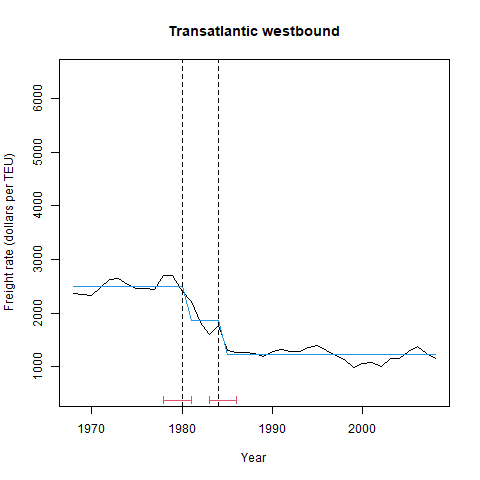
\includegraphics[keepaspectratio, scale=0.31]
  {figuretable/structural_change_transatlantic_westbound_before_2008.png}
  \end{minipage}
  \begin{minipage}[b]{0.3\linewidth}
  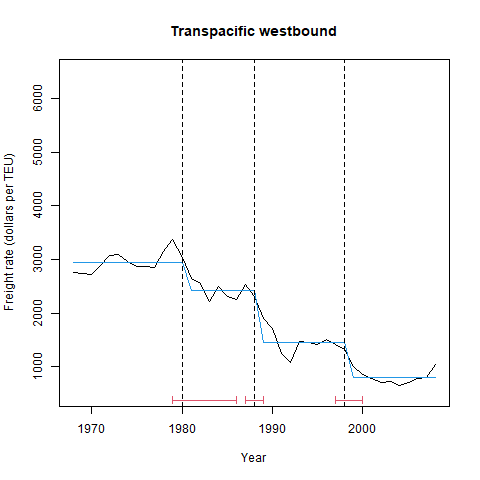
\includegraphics[keepaspectratio, scale=0.31]
  {figuretable/structural_change_transpacific_westbound_before_2008.png}
  \end{minipage}
  \begin{minipage}[b]{0.3\linewidth}
  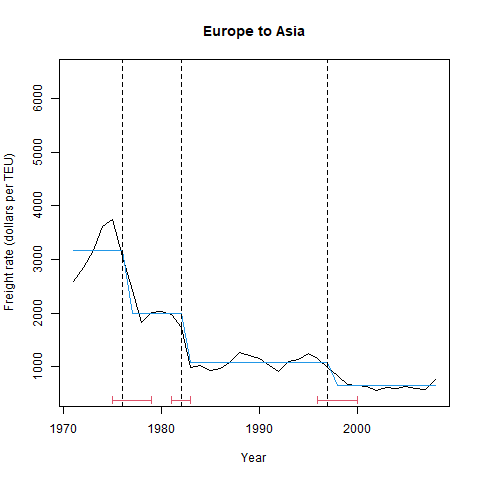
\includegraphics[keepaspectratio, scale=0.31]
  {figuretable/structural_change_europe_to_asia_before_2008.png}
  \end{minipage}\\
\begin{minipage}[b]{0.3\linewidth}
  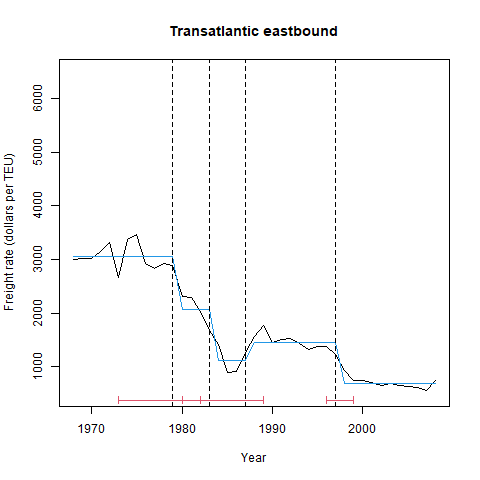
\includegraphics[keepaspectratio, scale=0.31]
  {figuretable/structural_change_transatlantic_eastbound_before_2008.png}
  \end{minipage}
  \begin{minipage}[b]{0.3\linewidth}
  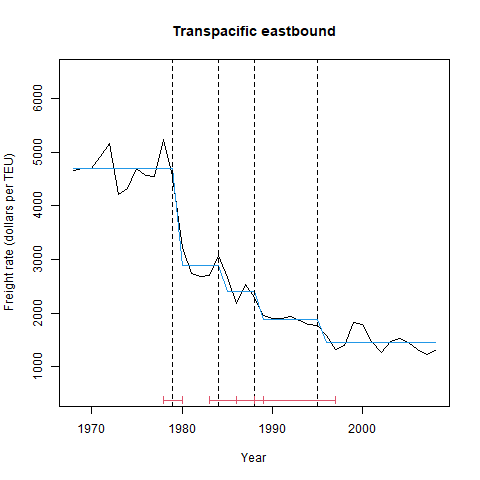
\includegraphics[keepaspectratio, scale=0.31]
  {figuretable/structural_change_transpacific_eastbound_before_2008.png}
  \end{minipage}
  \begin{minipage}[b]{0.3\linewidth}
  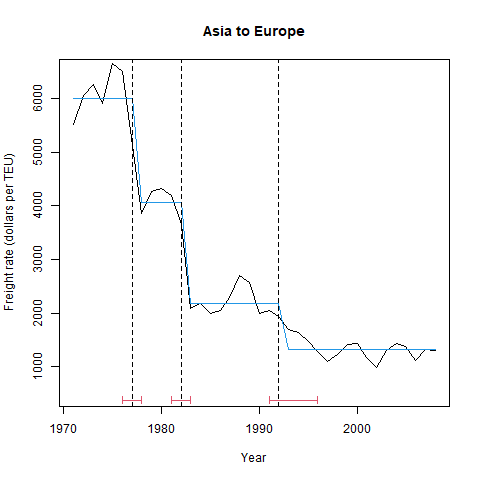
\includegraphics[keepaspectratio, scale=0.31]
  {figuretable/structural_change_asia_to_europe_before_2008.png}
  \end{minipage}
  {\scriptsize{}
  
\begin{tabular}[t]{llllllllll}
\toprule
  & BIC ($m$ = 0) & 1 & 2 & 3 & 4 & 5 & 6 & 7 & 8\\
\midrule
Transatlantic westbound & 647.86 & 555.88 & 538.08 & 538.1 & 538.89 & 538.95 & 545.65 & 552.91 & 560.26\\
Transatlantic eastbound & 685.71 & 620.56 & 596.29 & 582.23 & 581.03 & 584.06 & 587.28 & 592.78 & 598.48\\
Transpacific westbound & 679.59 & 609.32 & 592.63 & 568.14 & 568.96 & 573.59 & 579.5 & 586.58 & 593.87\\
Transpacific eastbound & 714.7 & 640.64 & 599.18 & 592.7 & 592.22 & 595.82 & 600.01 & 606.82 & 614.56\\
Asia to Europe & 684.17 & 620.42 & 593.91 & 567.82 & 571.46 & 576.96 & 584.01 & 591.2 & 627.68\\
\addlinespace
Europe to Asia & 631.38 & 581.33 & 553.76 & 539.17 & 545.08 & 551.75 & 558.62 & 566.59 & 588.79\\
\bottomrule
\end{tabular}

\caption{The estimated breakpoints and 95 \% confidence intervals with BIC.}
\label{fg:structural_change_transatlantic_eastbound_before_2008}
\begin{tablenotes}
\item[a]Note: Each segment shows the estimated breakpoints and the 95\% confidence intervals for $\hat{T}_i$ for $i=1,\cdots,4$ for each route. Following \cite{bai2003computation}, the number of breakpoints is selected by minimizing the BIC, as shown in the bottom table. The estimated parameters $\hat{\delta}_j$ and the standard errors for all $j=1,\cdots,k+1$ for all possible numbers of breakpoints are omitted. We use the sample between 1968 and 2008 for the Transatlantic and Transpacific routes and the sample between 1971 and 2008 for the Asia-Europe routes. We used the \texttt{strucchange} R-package developed by \cite{zeileis2002strucchange}.
   \end{tablenotes}
   }
\end{figure}

Figure \ref{fg:structural_change_transatlantic_eastbound_before_2008} illustrates the estimated breakpoints $\hat{T}_j$ and 95\% confidence intervals for route-year-level analysis of the shipping price. The bottom table shows the BIC for all possible numbers of breaks under $h=4$, where the minimizer of BIC is the optimal break number $\hat{k}$. First, we find that 95\% confidence intervals of the structural break cover the period between 1979 and 1980 on the U.S. routes (left and center panels), whereas the intervals cover the period between 1976 and 1978 on the non-U.S. routes (right panels). This indicates that the container crisis occurred on all six routes by 1980, which was triggered by the withdrawal of Sea-Land, although non-U.S. routes reacted earlier than U.S. routes. The reason for the response in non-U.S. routes seems to be related to reopening of the Suez Canal in 1976, which increased supply of container shipping services \citep{jsme2022}.

Second, we find remarkable differences between US routes and non-U.S. routes between 1984 and 1990. The 95\% confidence intervals of the structural break cover some period between 1984-1990 on the US routes, whereas there were no breaks on the non-US routes in the period. This implies that the enactment of the Shipping Act of 1984 generated some structural breaks in the treatment group, that is, the U.S. routes. Surprisingly, we also find that container crisis lasted heterogeneously even along the U.S. routes. For example, Transpacific routes seemed to recover in 1986, whereas Transatlantic routes were sour until 1990. This result may support the fact that the supply-demand relationship on the Transpacific and Transatlantic routes changed differently in the late 1980s. The substantial change in exchange rates after the Plaza Accord in 1985 led to a recovery in demand for transportation on the Transpacific route. On the other hand, no such situation was observed between Europe and the U.S.





\subsection{Industry-year-level newbuilding, secondhand, and scrap prices data}


\begin{figure}[!ht]
\centering
\begin{minipage}[b]{0.3\linewidth}
  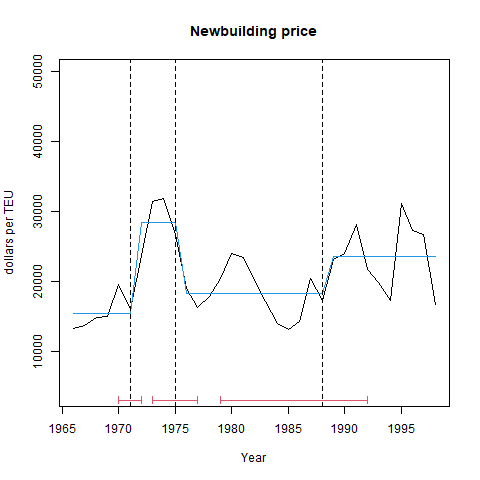
\includegraphics[keepaspectratio, scale=0.31]
  {figuretable/structural_change_newbuilding_price_before_1998.png}
  \end{minipage}
  \begin{minipage}[b]{0.3\linewidth}
  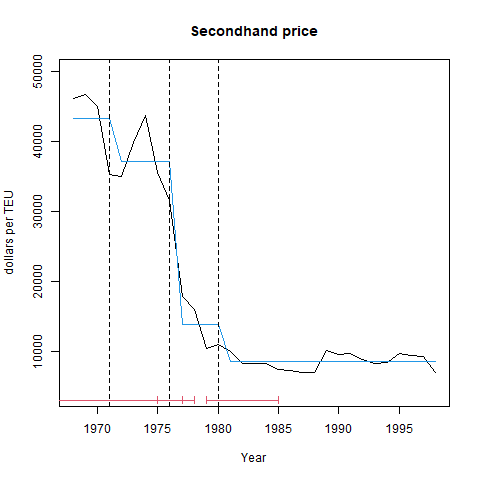
\includegraphics[keepaspectratio, scale=0.31]
  {figuretable/structural_change_secondhand_price_before_1998.png}
  \end{minipage}
  \begin{minipage}[b]{0.3\linewidth}
  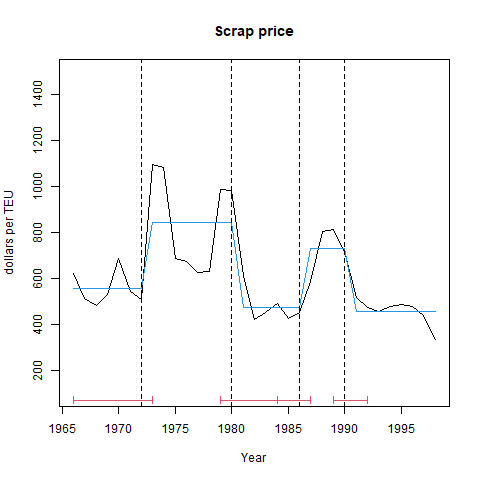
\includegraphics[keepaspectratio, scale=0.31]
  {figuretable/structural_change_scrap_price_before_1998.png}
  \end{minipage}
  {\scriptsize{}
  
\begin{tabular}[t]{lllllllll}
\toprule
  & BIC ($m$ = 0) & 1 & 2 & 3 & 4 & 5 & 6 & 7\\
\midrule
Newbuilding & 668.45 & 660.97 & 652.67 & 640.37 & 641.31 & 646.09 & 652.5 & 682.36\\
Secondhand & 687.84 & 613.29 & 613.68 & 612.51 & 618.38 & 623.22 & 629.53 & -\\
Scrap & 448.16 & 446.64 & 440.37 & 443.81 & 440.36 & 446.38 & 452.99 & 470.14\\
\bottomrule
\end{tabular}

\caption{The estimated breakpoints and 95 \% confidence intervals with BIC.}
\label{fg:structural_change_scrap_price_before_1998}
\begin{tablenotes}
\item[a]Note: Each segment shows the estimated breakpoints and the 95\% confidence intervals for $\hat{T}_i$ for $i=1,\cdots,4$ for each route. Following \cite{bai2003computation}, the number of breakpoints is selected by minimizing the BIC, as shown in the bottom table. The estimated parameters $\hat{\delta}_j$ and the standard errors for all $j=1,\cdots,k+1$ for all possible numbers of break points are omitted. We used a sample from 1968 to 1998. We used \texttt{strucchange} R-package developed by \cite{zeileis2002strucchange}. 
   \end{tablenotes}
   }
\end{figure}


Figure \ref{fg:structural_change_scrap_price_before_1998} illustrates the estimated breakpoints $\hat{T}_j$ and 95\% confidence intervals for industry-level analysis of newbuilding, secondhand, and scrap prices. First, we find that 95\% confidence intervals of the structural break cover the period between 1974 and 1976 for newbuilding and secondhand prices. These results correspond with the shipping price trend of the Asia-Europe market. Second, downward structural breaks in all prices were not detected between 1984 and 1990. These results imply that the container crisis did not significantly decrease industry-level prices in the shipbuilding market, unlike route-level shipping prices. We interpret these differences as naturally capturing the differences between shipping markets with shipping conferences and shipbuilding markets without cartel groups.

\section{Discussion, Practical implication, and Future Research}

[Discussion 1 paragraph] We summarize 

[Practical implication 1 paragraph]

[Future research 1-2 paragraph]


\section{Conclusion}\label{sec:conclusion}
This study provides a new unified panel dataset of route-year-level freight rate and shipping quantity in the six major routes and industry-year-level newbuilding, secondhand, and scrap prices from 1966 (beginning of the industry) to 2009. The data is a fundamental basis for understanding the container shipping industry. The data and structural break tests provide historical insights into the nonstationary dynamics of these price variables, known as the container crisis. We found that the container crisis was a specific event in the shipping market. Our data sheds light on the industry dynamics with shipping cartels. We leave detailed analysis based on the data for future work. 

\textbf{Acknowledgement} \\
We benefited from anonymous referees and seminar participants at the International Association of Maritime Economists 2022. We thank Akimitsu Ashida and Hiroyuki Sato for sharing industry knowledge and expertise as ex-chairperson in the 1980s. This study was supported by JSPS KAKENHI Grant Numbers 20K22129 and 22K13501. 


\bibliographystyle{aer}
\bibliography{ship_bib}

\appendix
\begin{landscape}
{
\begin{table}[htb]\centering
{\tiny{}
  \begin{tabular}{lllll}
  Container Price & Year & Source & Measured Units & Note\\\hline
               & 1965,1970,1975,1979 & Issues of Our Ocean Shipping &dollars per 100 tons-mile&Liner sector, three main cargo\\
               & 1973-1976 & Current status of marine transportation &converted dollars per TEU&Revenue and quantity on only Transpacific and Asia-Europe routes\\
               &1976-1994 & Global Container Markets Drewry Shipping Consultants &dollars by FEU &Missing 1976-1989 in Asia-Europe\\
               &1994-2009 & Review of Maritime Transport &dollars by TEU&All market-level info is available\\
              & & & &\\
  Liner price & & & &\\\hline
               &1965-2009 & Review of Maritime Transport &index rate based on 1995(=100)&Global liner freight rate\\
               & & & &\\
  Quantity & & & &\\\hline
                    &1966-1972 & Containerization International 1973&TEU& Aggregate carrying capacity for each route\\
                    &1970,1974,1978,1980 &The Container Crisis 1982 &1 million ton&
                    Aggregate quantity for each route\\
                    &1975,1978,1981,1984,1987,1990&Container transportation cost and profitability 1980/2000 &1000TEU&Aggregate quantity for each route\\
                    &1985-1997&World Sea Trade Service &1000TEU&All market-level info is available\\
                    &1994-2009 & Review of Maritime Transport &1000TEU& All market-level info is available\\
                     & & & &\\
                    &(1970,1975,1977,1978,1979) &*Issues of Our Ocean Shipping &D/W tons&Aggregate quantity for each route\\
                    &(1973)& *Containerization International 1975 &1000TEU&Aggregate quantity for each route\\
                    &(1978,1981)&*The Container market to 1990 &TEU&Aggregate carrying capacity for each route and container type\\
                    &(1983)&*World Container Data 1985 &1000TEU&Aggregate quantity for each route
  \end{tabular}
  \begin{tablenotes}
\item[a]\textit{Note:} The data sources with ($*$) are used for reference to check the consistency of the trend.
\end{tablenotes}
  }
  \caption{Overview of data sources.}
  \label{tb:overview_of_datasources}
\end{table}
\begin{figure}[!ht]
\begin{minipage}[b]{0.45\linewidth}
  \centering
  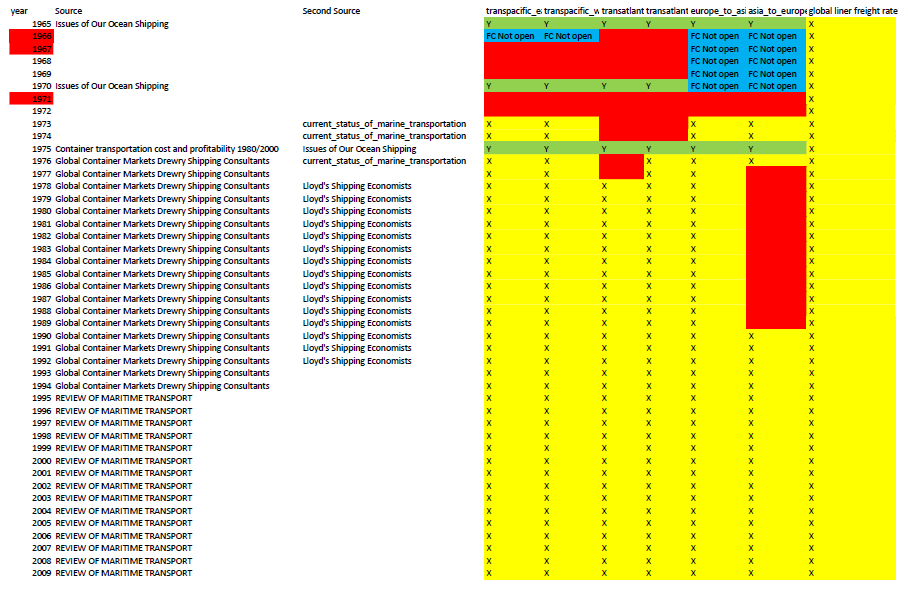
\includegraphics[height = 0.4\textheight]{freight_rate_filled_and_imputed_summary.png}
  \end{minipage}
  \begin{minipage}[b]{0.45\linewidth}
  \centering
  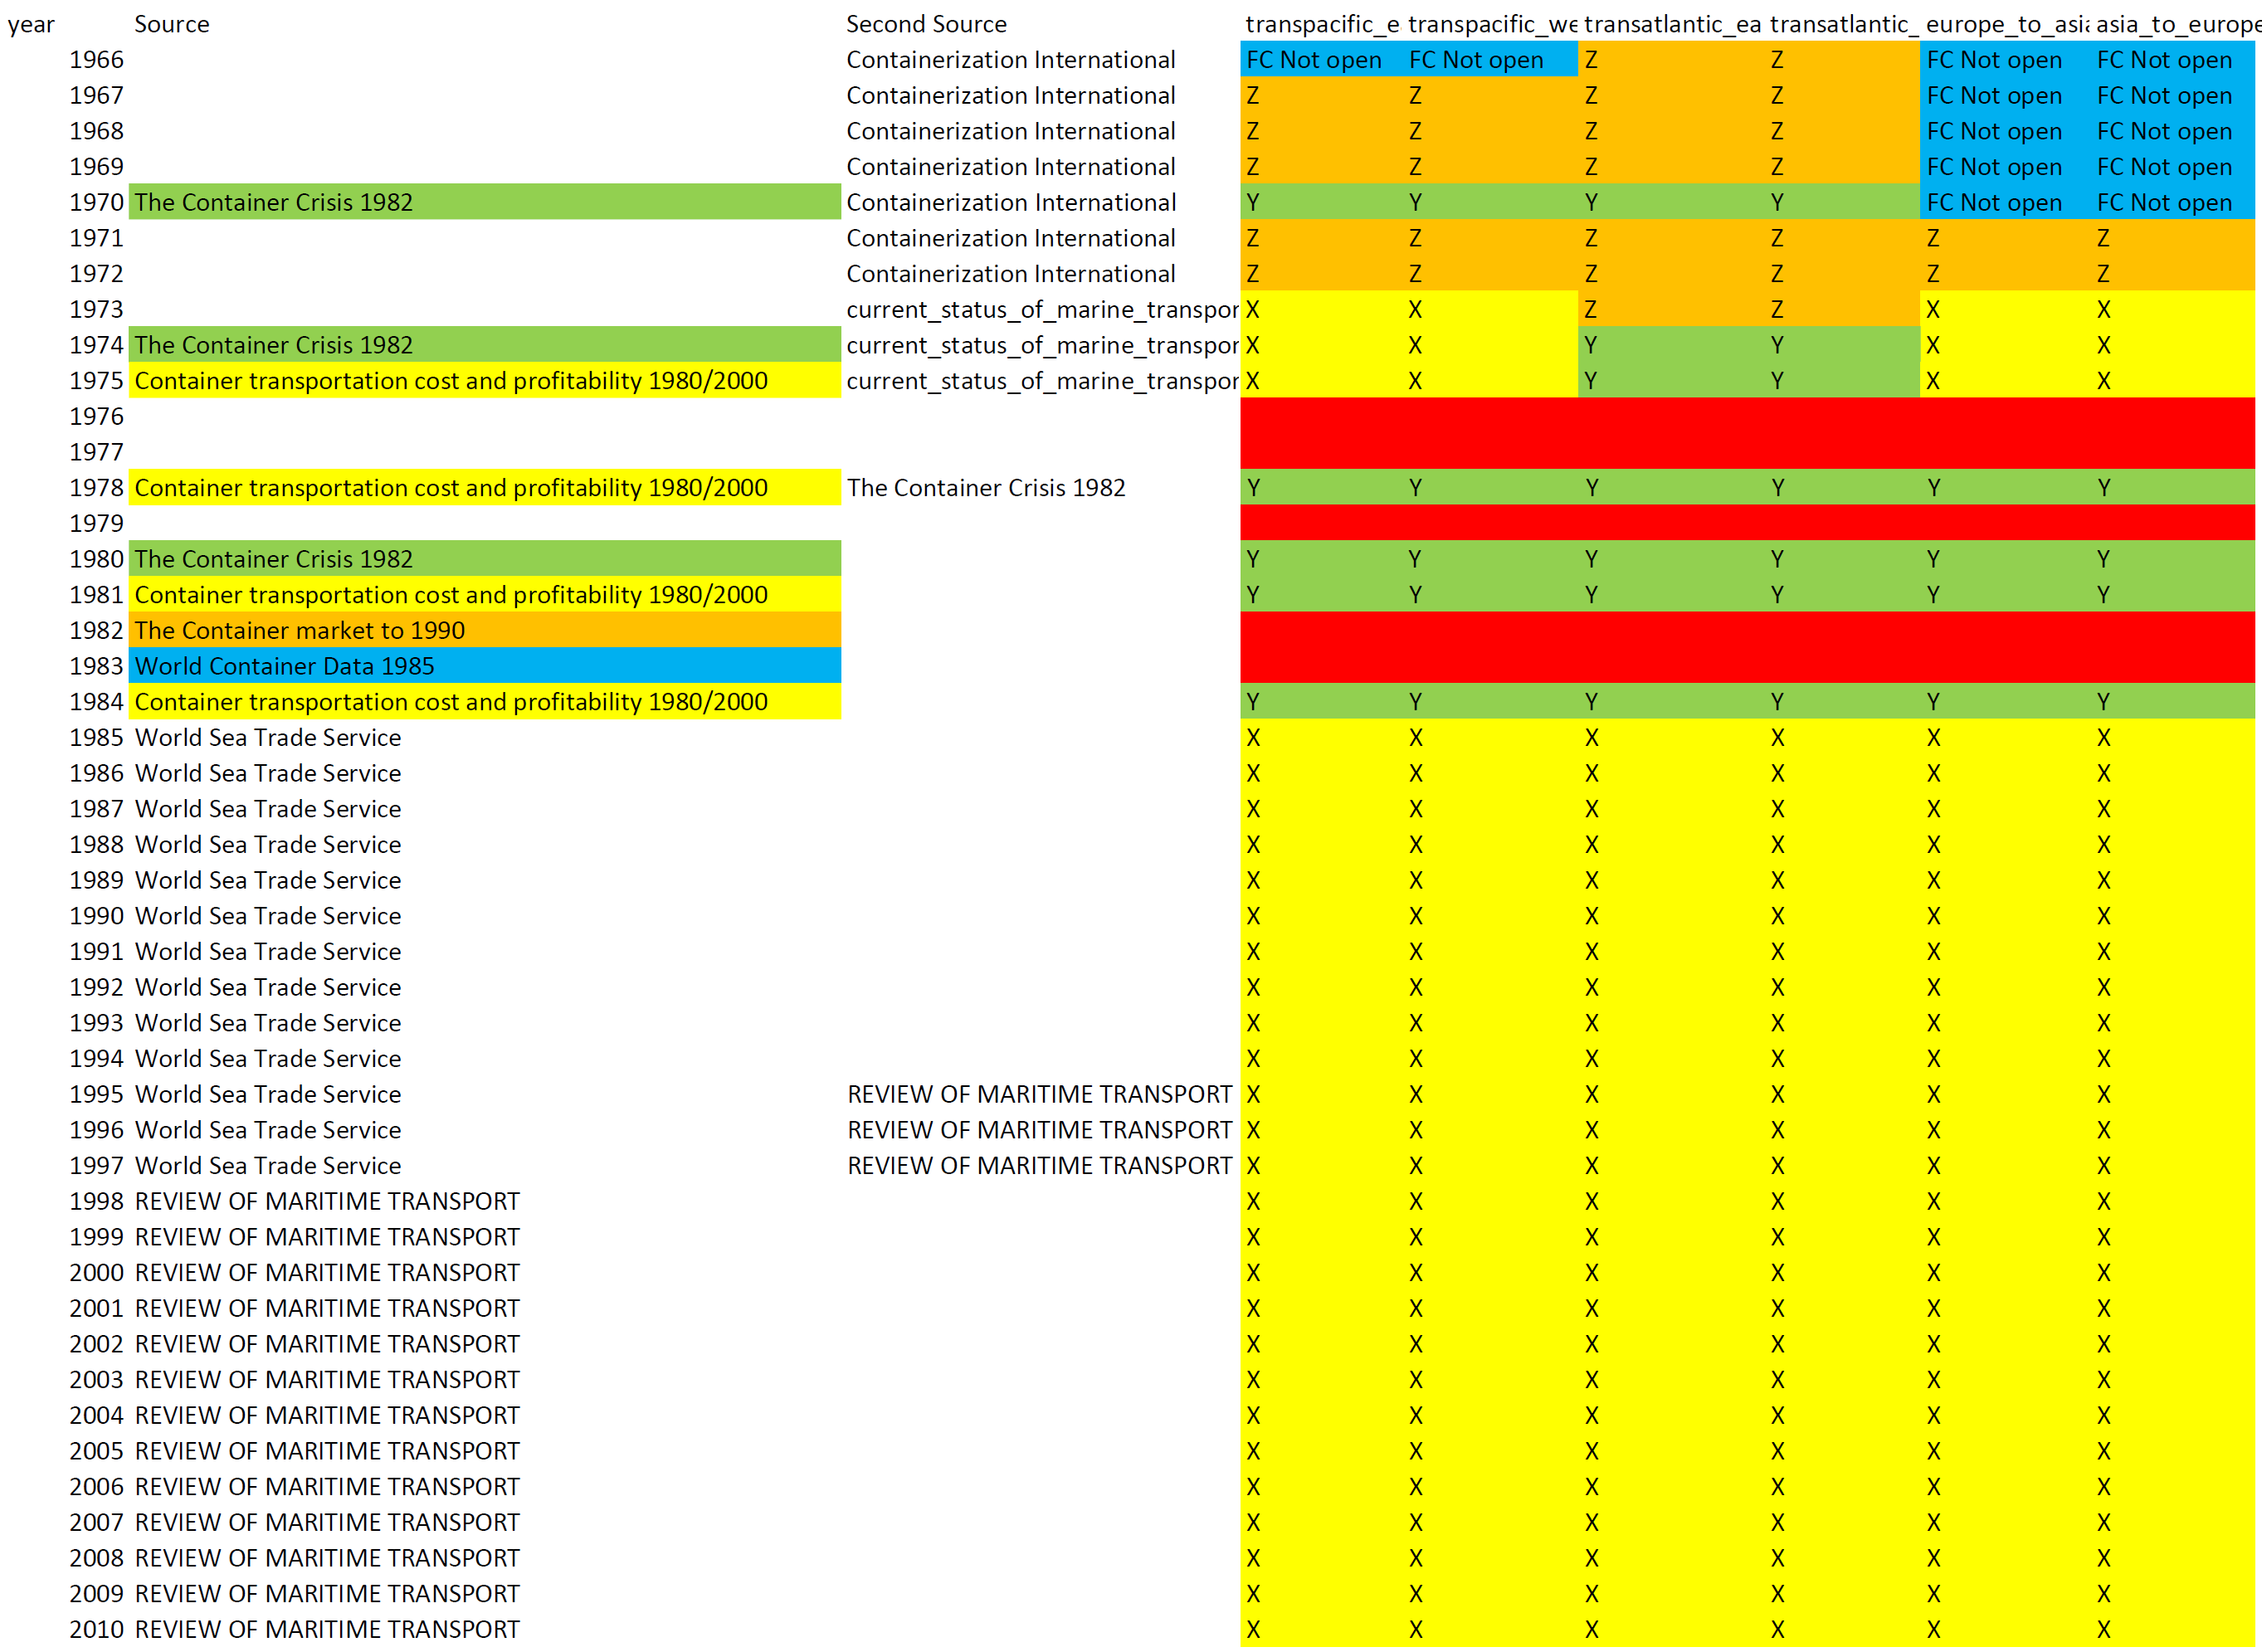
\includegraphics[height = 0.4\textheight]{traffic_amount_filled_and_imputed_summary.png}
  \end{minipage}
\caption{The observed and imputed variable cells for market-level data.}
{\tiny{}
\begin{tablenotes}
\item[a]\textit{Note:} In the yellow X cells, the route-level variables are recorded in data. In the green Y cells, the route-level cells that cannot identify the eastbound and westbound routes are recorded, so that we assign the the values based on the fixed ratio of the eastbound to the westbound in the closest period. In the orange Z cells, although route-level variables are not recorded, ship-level variables with targeted routes are available, so that we convert firm-level information into route-level variables based on the fixed ratio in the closest period. The red cells are missing values. Thus, we impute the values via interpolation based on the observed points in each route and global liner freight rate.
\end{tablenotes}
}
\end{figure}
}
\end{landscape}

\section{Data construction (Not for publication)}\label{sec:data_construction}

The container shipping industry is a fascinating laboratory for investigating industry dynamics. Because the industry started global shipping in 1966, we can find the initial state of the market dynamic structure. There is also substantial firm entry and exit in the industry, which makes the container shipping industry ideal for studying industry dynamics in global markets. Finally, the markets see the dynamics of shipping alliance, mergers, and consolidations. 

Despite the significance, a panel dataset regarding the container freight rate and shipping quantity on the three major trade routes (front-haul and back-haul separately) between 1966 and 2009 has not been available. \footnote{Similar to related papers focusing on the container freight rate panel data, \cite{luo2009econometric} use shipping demand and freight rate data between 1980 and 2007. As shipping demand, they used the world container throughput reported in the Drewry Annual Container Market Review and Forecast. The container freight rate, which is calculated as the weighted average of Transpacific, Europe-Far East and Transatlantic trades from the same data source. Because of the data limitation, they calculated the missing period (1980–1993) from the General Freight Index in the Shipping Statistics Yearbook 2007, using a simple statistical equation between container freight rate and the general freight index from 1994 to 2008.}  This note provides unified instruction and guidance to construct the dataset based on published books and publicly available data sources as much as possible, although the construction and merging processes will involve conversion and imputation errors from multiple datasets. The data sources are presented in Table \ref{tb:overview_of_datasources}. Instead of manually constructing the freight index from the commodity-level freight rate via formal but complicated processes, we adopted the tractable imputation approach, that is, linking multiple data sources that overlap information for a few years. The corresponding code is also provided to ensure that an interested researcher can replicate the construction. 

Collecting data on the container freight rate and shipping quantity, particularly before 1994, is not trivial because there is no single data source. In the subsequent subsections, we have provided detailed data construction for each container freight rate and shipping quantity.

\subsection{Container freight rate}

To construct the data regarding the container freight rate, we refer to the three data sources presented in Table  \ref{tb:overview_of_datasources} and the liner freight rate before global containerization.

\subsubsection{Shipping alliance and Liner freight rate}\label{subsec:shipping_alliance}

The liner shipping industry has traditionally formed shipping alliances like explicit cartels. Until 1984, shipping alliances played an important role in the container-shipping market. For example, in February 1967, a container shipping firm, Matson, started an operation on the Atlantic route under the freight rate contracted with one of the alliance groups, the TPFC. Thus, the container freight rate was determined by liner shipping alliances.

This unique feature allows us to use the liner freight rate to approximate the container freight rate. Figure \ref{fg:liner_freight_rate} compares the liner freight rate with the container freight rate recorded since 1995. This suggests that the container freight rate and its fluctuations can be inferred from the liner freight rate. In particular, “Issues of Our Ocean Shipping” recorded that in 1978, 76.0\%  of U.S. liner transports, 66.4\% of European liner transports, and 68.8\% of Asian and Australian liner transports were containerized. That is, more than two-thirds of the liner freight rate was determined by the container freight rate in the 1970s, as in the 1990s.


\begin{figure}[!ht]
\begin{center}
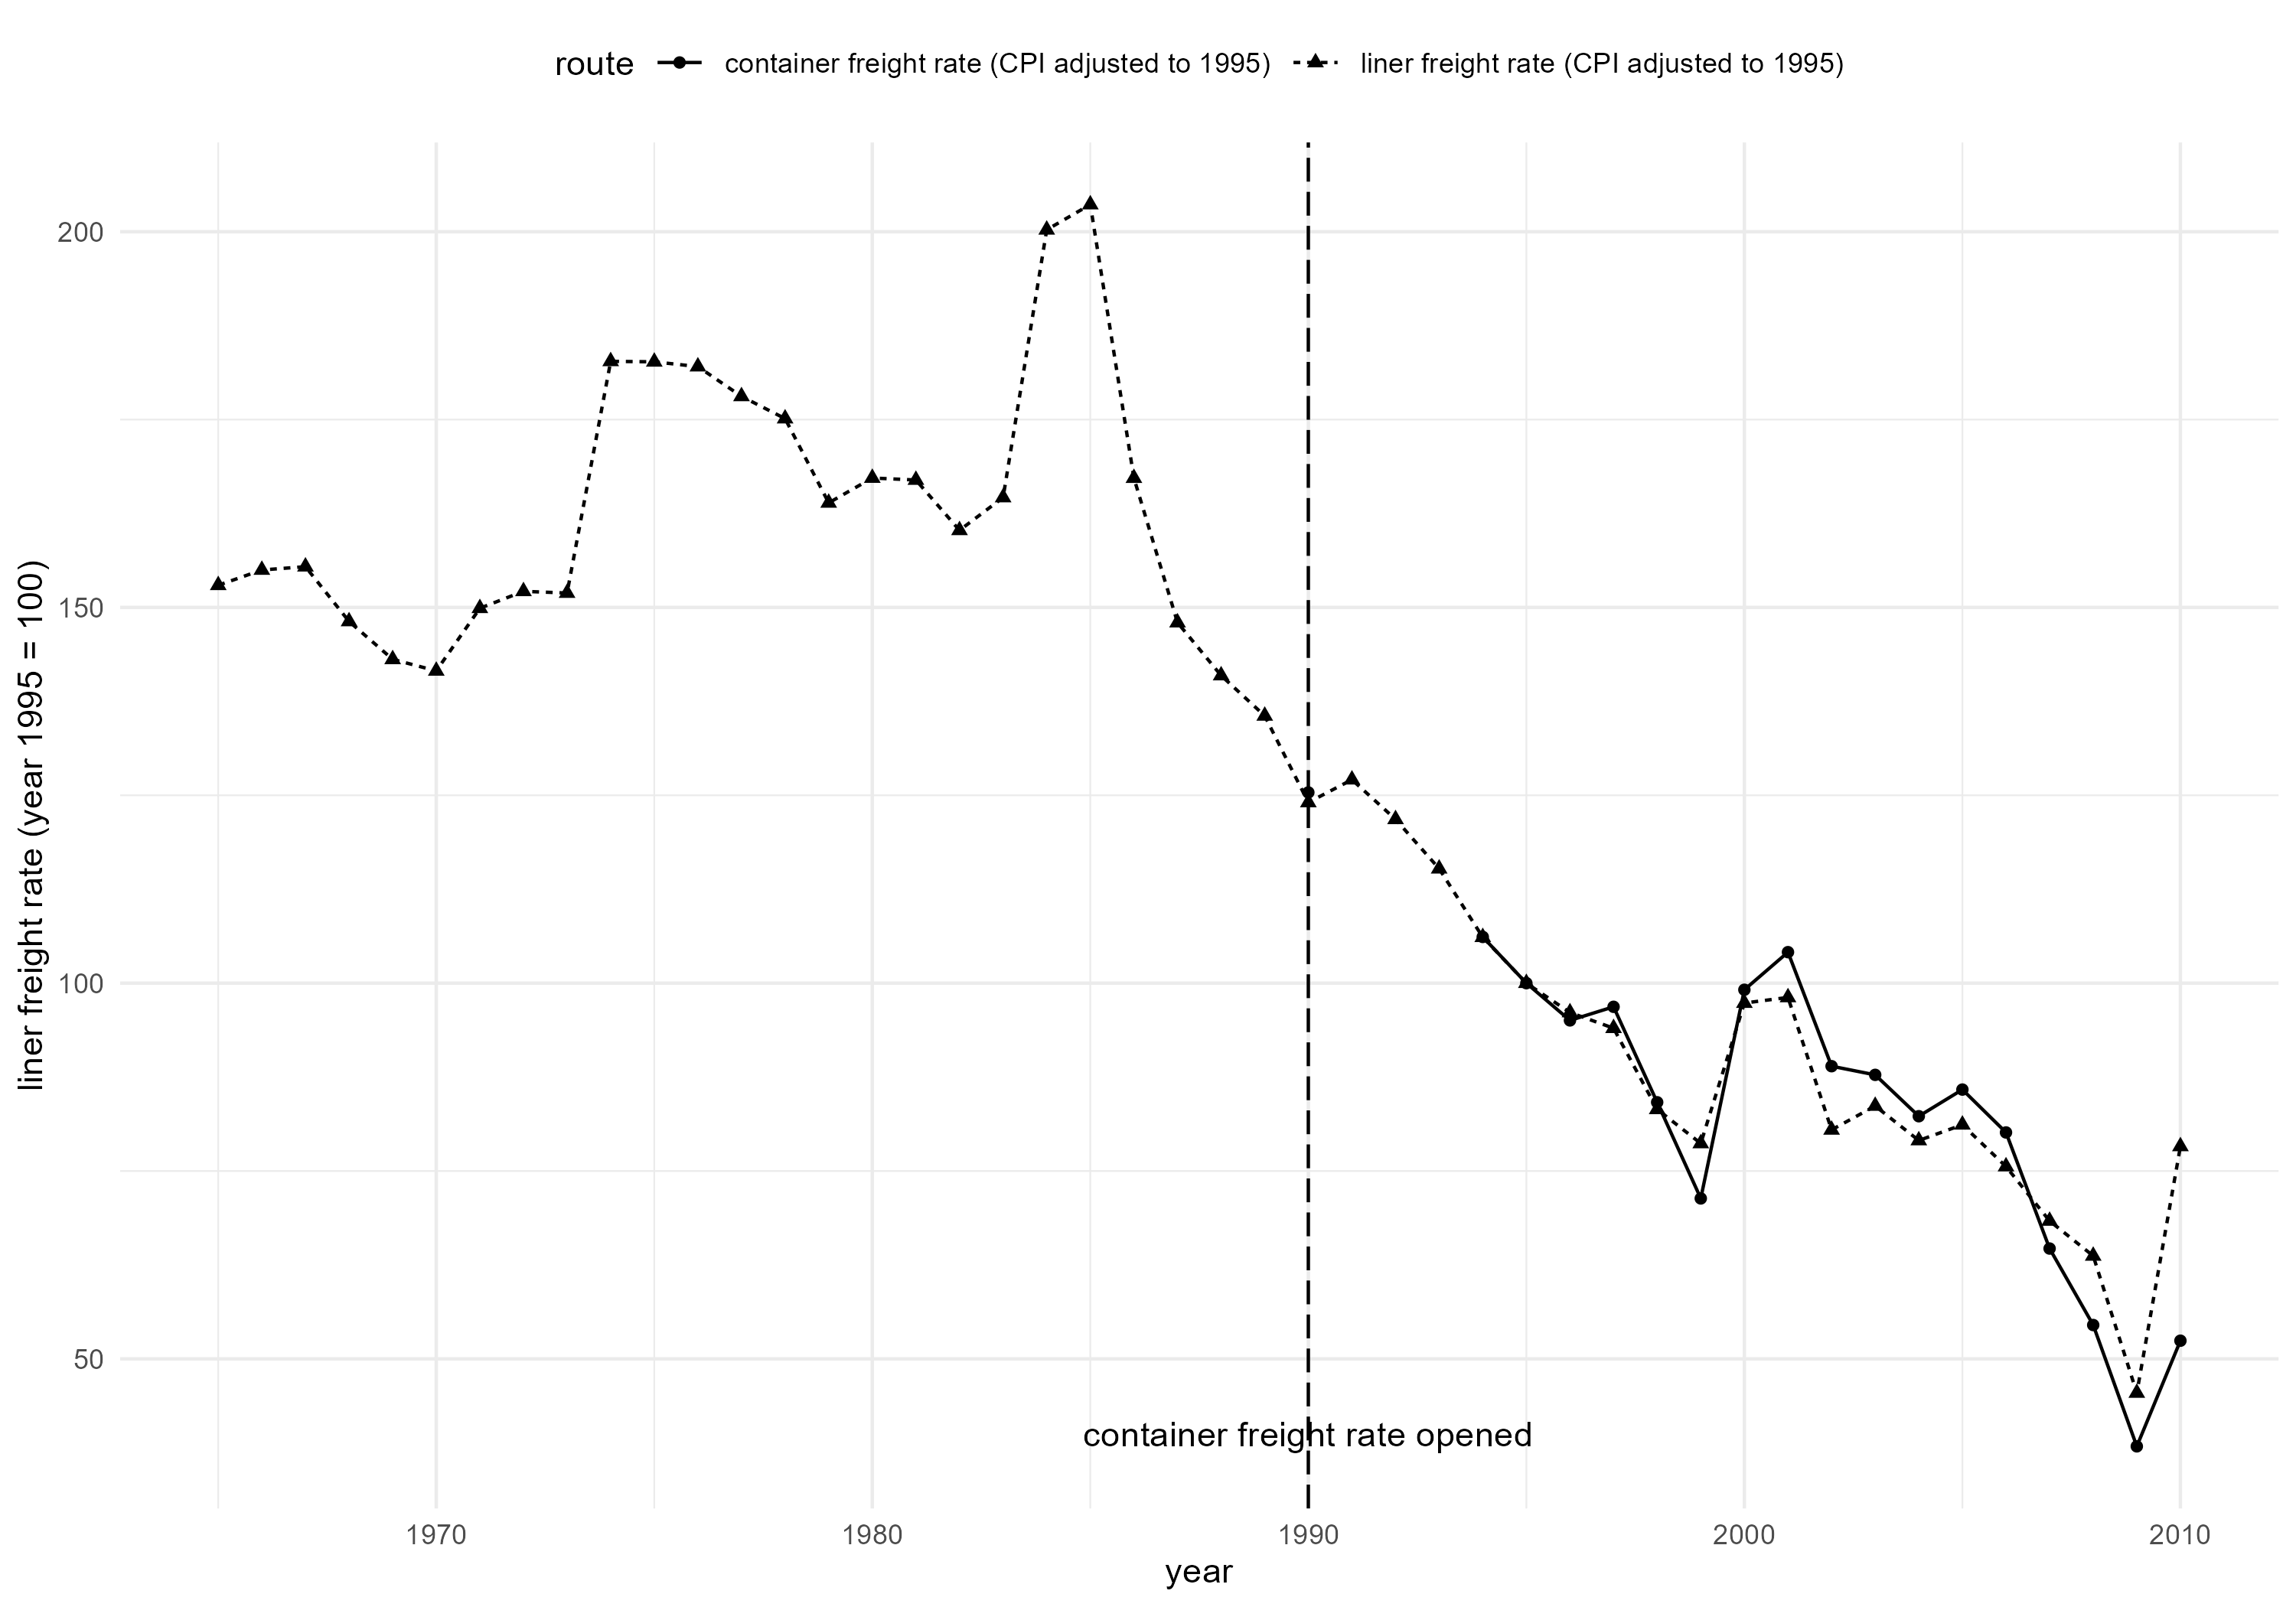
\includegraphics[height = 0.4\textheight]{figuretable/liner_freight_rate.png}
\end{center}
\caption{The trend of the liner freight rate.}
\begin{tablenotes}
\item[a]\textit{Note:} Source: \textit{Review of Maritime Transport}, published annually by UNCTAD. The measure of the price index is not explicitly mentioned in the Review of Maritime Transport.
\end{tablenotes}
\label{fg:liner_freight_rate}
\end{figure}


\subsubsection{Container freight rate between 1966 and 1975}



Data on the freight rate between 1966 (i.e., the beginning of the industry) and 1975 are missing from a single data source. Thus, we need to infer and impute data from multiple data sources and information in subsequent years. Fortunately, we can use the institutional knowledge in Section  \ref{subsec:shipping_alliance}, the liner freight rate, and the published data that overlap the data in some subsequent years in multiple data sources.

``Issues of Our Ocean Shipping" (\textit{``Wagakuni no Gaikou Kaiun Ni Tsuite", in Japanese}) records the freight rate of liner shipping on the three major routes in 1965, 1970, 1975, and 1979. The freight rates for the three types of cargo (i.e., electric appliances, clothes, and ceramic products) are available. These freight rates were measured in dollars for 100 tons per mile. The shipping miles between specific ports are listed.\footnote{For the Transpacific and Asia-Europe routes, the shipping miles between specific ports, that is, Japan-Hamburg and Japan-San Francisco routes are mentioned. However, only for the transatlantic route, the specific ports were not mentioned. Thus, we take the average of the shipping miles for Hamburg-San Francisco (i.e., west coast) and Hamburg-Halifax routes (i.e., east coast).} Using this information, we can recover the route-level container freight rates for 1965, 1970, and 1975. Finally, we assumed that the proportions of the liner and container freight rates for each route were fixed before 1975. Under this assumption, we recovered and interpolated the eastbound and westbound container freights for each route based on the fixed proportion of the liner and container freight rate and that of subsequent years, which overlaps container freight rates in multiple data sources. \footnote{The overlapped information in 1979 is a key year for merging multiple data before and after 1975. However, the freight rate swung irregularly and non-proportionally in both data sources. For making the smooth transition of the freight rate in the merged dataset, we calculated the conversion rate based on the freight rate of 1975 from \textit{Issues of our ocean shipping} and that of 1976 from \textit{Global container markets year}.}



\subsubsection{Container freight rate between 1976 and 1994}

The container industry faced significant market changes during this period. Specifically, in 1984, the maritime cartel was applied to the United States’ antitrust law to ensure the determinants of the liner freight rate changed. After 1984, it approached a competitive global market.

The data on the freight rate between 1976 and 1994 were recorded in \textit{Global Container Markets Drewry Shipping Consultants}. The recording of the freight rate starts from 1976 for the transatlantic and Transpacific routes and from 1990 for the Europe-Asia route. Thus, data on the freight rate of the Europe-Asia route between 1976 and 1989 are missing.\footnote{\textit{Global Container Markets Drewry Shipping Consultants} stated that, ``the Europe-Far East trade is the least well documented of the axial routes (page 109)".} 

For the imputation of the missing data, we assumed that the proportion of liner and container freight rates for eastbound and westbound Asia-Europe routes are fixed between 1976 and 1990. This assumption implies that there is no time-varying difference between the eastbound and westbound Asia-Europe routes. Under this assumption, we recovered the container freight rates of the eastbound and westbound Asia-Europe routes.



\subsubsection{Container freight rate after 1995}\label{subsec:freight_rate_after_1995}

The freight rate data are recorded in the  \textit{Review of Maritime Transport} which refers to \textit{Containerization International Yearbook}. The recording of freight rates began in June 1994.\footnote{\cite{jeon2022learning} stated: ``The first dataset on firm-level investment and capital is therefore supplemented with the historical price and quantity data compiled from the Review of Maritime Transport published by the United Nations that goes back to 1997." (p. 9). However, we confirm that the data in 1994 are available in \textit{Containerization International Yearbook}.} \textit{Containerization International Yearbook} mentioned that \textit{``the information is derived mainly from confidential reports provided by some of the main carriers and other public sources."} Owing to the consistency of data sources and public availability, the \textit{Review of Maritime Transport} is often used. For example, \cite{jeon2022learning} used quarterly freight data.


Processing the above steps generate the time-series data of the container freight rate for each route between 1966 and 2009. Figure \ref{fg:container_freight_rate_each_route} reveals the trend of the container freight rate, CPI-adjusted to 1995, with the liner freight rate depicted in Figure \ref{fg:liner_freight_rate}. In particular, the recovered and imputed data points in the 1960s and the 1970s quantitatively captured anecdotal and institutional evidence. First, for the transatlantic and Transpacific routes, the peak in 1976 and a sharp declining trend in 1979 were captured. Second, the container freight rate on each route corresponds to  the fluctuation of the liner freight rate.

\begin{figure}[!ht]
\begin{center}
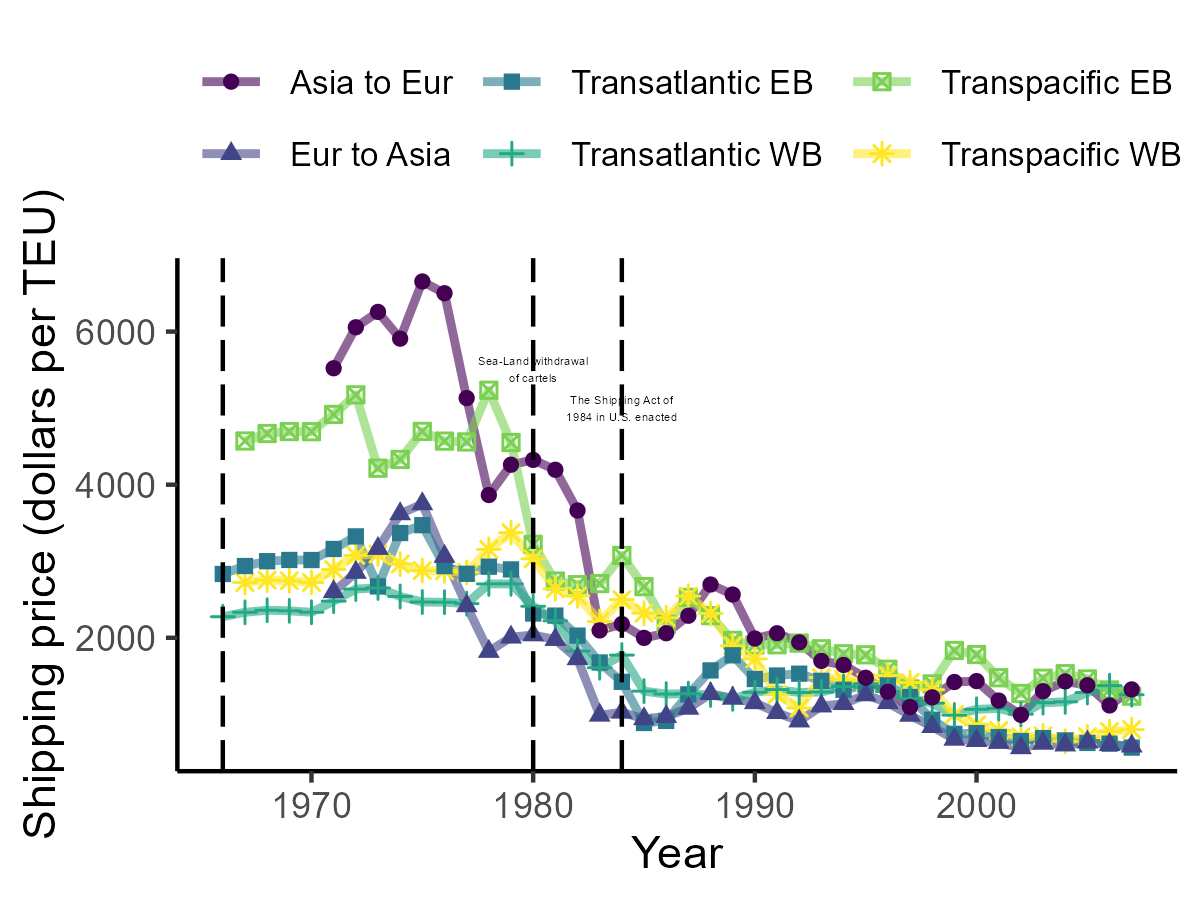
\includegraphics[height = 0.5\textheight]{figuretable/container_freight_rate_each_route.png}
\end{center}
\caption{The trend of the container freight rate.}
\label{fg:container_freight_rate_each_route}
\end{figure}

\subsection{Shipping quantity}

To construct data regarding the container trade volume, we refer to five data sources shown in Table \ref{tb:overview_of_datasources}.

\subsubsection{Shipping quantity between 1966 and 1975}

Official data on shipping quantities between 1966 and 1969 were not available. However, we could keep track of the development of container vessels during this period. First, data regarding vessel capacity were recorded in \textit{Containerization International 1973}.\footnote{``Theory and Practice of Container Shipping" (\textit{``Container Yusou no Riron to Jissai", in Japanese}). This contains the information about the launch of container ships owned by the United States main four firms, Moore-McCormack, U.S. Lines, SeaLand, and CML (American Export Isbrandtsen). This help me to identify the exact launch year only of full-container ships by the largest players, that is, United States container shipping companies. We use the data source only to check institutional evidence.} This information identifies the carrier composition on the Transatlantic, Transpacific, and Asia-Europe routes between 1966 and 1972.

Second, \textit{Review of Maritime Transport} (1971) summarizes the relationship between the annual global container carrying capacity and container capacity in 1969 and 1970 on the transatlantic route. We assume that container capacities were fully exploited during this period. This assumption is not restrictive, because the demand for container shipping was considerably high during this period. Under this assumption, the shipping quantity is recovered by calculating the total shipping quantity from the container capacity and invariant conversion rate.

% \begin{table}[ht!]
% {\tiny{}
%     \centering
%     \begin{tabular}{ccllll}
%       Year &page& Event & Firm (Group) & annual global capacity (TEU) & container capacity (TEU) \\\hline
%       Transatlantic route && &  & &\\
%       1966, Feb && 6 semi-containers& by Moore-McCormack & &\\
%       1966, Mar & p.27& 4 semi-containers& by U.S. Lines & &\\
%       1966, Apr &p.29& 4 full-containers& by SeaLand & & 0.5 million tons\\
%       1966, Sep &p.29& 4 full-containers& by CML (American Export Isbrandtsen) & & 0.4 million tons\\
%       &&&&&\\
%       1967, Sep &p.194& 3 Ro-Ro ships &by ACL & &0.75 million tons\\
%       &&&&&\\
%       1968, Feb &p.194 & 5 full-containers &by U.S. Lines & &0.65 million tons\\
%       1968, Sep &p.194 & 6 full-containers &by Sealand & &3 million tons\\
%       1968,??? &p.74 & 5 full-containers &by U.S. Lines & &?\\
%       1968,summer &p.76 & 3 full-containers &by CML (American Export Isbrandtsen) & &?\\
%       &&&&&\\
%       1969 &RMT(1971)& XX & & 66100 &714000\\
%       1970 &RMT(1971)&   & & 104700 &114200\\
%       &&&&&\\\hline
%       Tranpacific route && &  & &\\
%       1967, Sep && 7 ships &by Matson & &\\
%       && &  & &\\
%       1968, Sep && ? containers &by Japanese groups & &\\
%       && &  & &\\\hline
%       Asia-Europe route && &  & &\\
%       1970  && 1 full-container &by Nippon Yusen &&\\
%     \end{tabular}
%     \caption{The container industry historical background before 1970. Source: Review of Maritime Transport 1971.}
%     \label{tb:container_industry_history_before_1970}
% }
% \end{table}


Third, the data on shipping quantity in 1970 and 1974 were recorded in \textit{The Container Crisis 1982}, and the data for 1973 were recorded in \text{containerization international 1975}, fortunately. However, data for 1971 and 1972 were missing. The data also contains the regional levels of container shipping, that is, container traffic in Asia, North America, and Europe. One of the alternatives is the imputation approach, which employs external data that provide information about missing data.\footnote{\cite{jeon2022learning} stated that: “We set the start date for firms’’ information as the second quarter of 1966, which is the date of the first international container voyage. Then, we employed quarterly data on the value of trade by origin-destination pair from the IMF Direction of Trade Statistics database to impute the missing data on demand states from 1966: Q2-1996: Q4.” (p. 25), and “To translate the value of trade to the quantity of container trade, the demand state for the 1997–-2014 period was regressed on the de-trended value of trade. Then, the demand states for periods with missing data are constructed as predicted values from the regression. For the 1997–-2014 period, actual demand states are used.” (footnote 37).} We assign the recorded trade volume to each route in proportion based on the subsequent years.\footnote{Alternatively, we could assign the aggregate container shipping quantity to westbound and eastbound routes based on the data on the value of trade by origin-destination pair from \textit{the IMF Direction of Trade Statistics database}. We did not take the full-imputation approach because the value of trade includes goods transported by the bulk shipping service.} For missing years, we interpolate the trade volume using observed data points.



\subsubsection{Shipping quantity between 1976 and 1994}

The data on shipping quantity between 1976 and 1994 were recorded in \textit{World Sea Trade Service}, \textit{Container transportation cost and profitability 1980/2000}, \textit{The Container Crisis 1982}, and \textit{World Container Data 1985}. In particular, \textit{World Sea Trade Service} started recording data from 1985, whereas the other data sources recorded the data before 1985 but irregularly. Specifically, the quantity data for 1971, 1972, 1973, 1976, 1977, and 1979 were missing for all routes, and the quantity data for 1970, 1974, 1980, 1982, and 1983 are recorded in the total shipping quantity, summing up eastbound and westbound for each market.




\subsubsection{Shipping quantity after 1995}
The data about shipping quantity after 1995 are recorded in the  \textit{Review of Maritime Transport} and \textit{World's sea trades}. The former refers to \textit{World Sea Trade Service Review, various issues, 1996}, \textit{Journal of Commerce, various issues, 1996}, and \textit{Containerization International, various issues, 1996.} As in Section \ref{subsec:freight_rate_after_1995}, shipping quantity data are easily constructed from a single data source, that is, the  \textit{Review of Maritime Transport}. Before merging the data before and after 1995, we confirm that the discrepancy between the two data sources is small for almost all market-year observations. However, only the quantities in the transatlantic eastbound and westbound routes in 1995 were somewhat different.

Processing the above steps generate the time-series data of container shipping quantity measured by 1,000 TEU for each route between 1966 and 2009. Figure \ref{fg:container_shipping_quantity_each_route} illustrates the trend in container shipping quantity. The shipping quantity on all routes increased monotonically between 1973 and 2000. After 2000, this trend increased exponentially, particularly in the Transpacific eastbound and Europe-to-Asia routes.

\begin{figure}[!ht]
\begin{center}
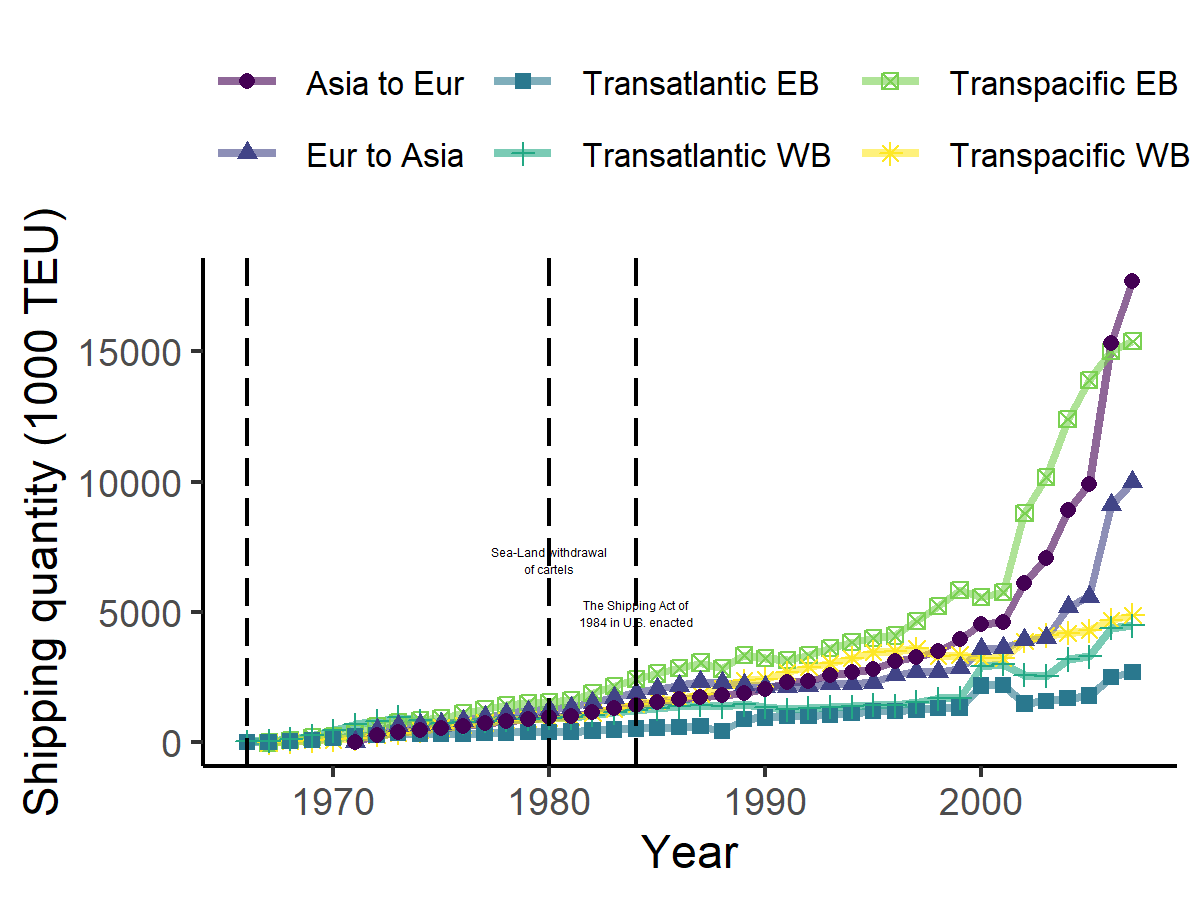
\includegraphics[height = 0.5\textheight]{figuretable/container_shipping_quantity_each_route.png}

\end{center}
\caption{The trend of the container shipping quantity. The trend before 1976 is based on ship-level carrying capacity information in each route.}
\label{fg:container_shipping_quantity_each_route}
\end{figure}


\subsection{Newbuilding, Secondhand, and Scrap prices}
We provide a recommendation for constructing newbuilding, secondhand, and scrap prices for container ships from 1967. Our data were collected from a series of \textit{Review (1971-1998)} published by Fearnley and \textit{Lloyd's Shipping Economist (1983-1990)} published by Lloyd's of London Press. 

\subsubsection{Newbuilding prices}
We collected industry-year-level newbuilding prices per 18000 DWT bulk ships from \textit{Review (1971-1998)}. ). Using the overlapped year, we converted the prices into consistent prices under the assumption that the conversion rate is invariant across years. Then, we divided the price per 12000 dwt by 10 to convert to the price per 1200 TEU and then converted it into the price per TEU. Finally, we converted bulk prices into container prices based on \textit{Lloyd's Shipping Economist (1983-1990)}.

\subsubsection{Secondhand prices}
We collected industry-year-level secondhand prices per 16000 DWT CSD (liner type) ships from \textit{Review (1971-1998)}. Using the overlapped year, we converted the prices into consistent prices under the assumption that the conversion rate is invariant across years.

We assume a fixed depreciation rate ($= X$) and fixed conversion rate ($= a$) for 1981 and 1983, and observe the following:
\begin{align*}
    1981: 2.7 + 2X &= 16.0a \quad\text{(18-year depreciation)}\\
    1983: 0.8 + 0X &=11a \quad\text{(20-year depreciation)}
\end{align*}
We solve the system of equation for $X$ and $a$. To obtain the price per $1600dwt+15X$, we multiplied the above price by 12000/16000 and obtained the price per 12000dwt. Then, we divided the price by 10 to convert it to the price per 1200TEU. We then converted it into the price per TEU of 5 years ship by dividing it by 1200. Finally, we converted the liner prices into container prices based on \textit{Lloyd's Shipping Economist (1983-1990)}.


\subsubsection{Scrap prices}

We collected industry-year-level scrap prices per LTD in the Far-East. Using the overlapped year, we converted the prices into consistent prices under the assumption that the conversion rate is invariant across years. We then divided per LTD by four to obtain the price per dwt, multiply it by 10, and convert it into the price per TEU.\footnote{The rate is based on \textit{https://nippon.zaidan.info/seikabutsu/2002/00264/contents/030.htm}.}


% \input{20test_for_parallel_trend}
% \input{21_estimate_conduct_parameter}

\end{document}